\documentclass{AeroStructure-ERJohnson}

\usepackage{dcolumn}
\newcolumntype{d}[1]{D{.}{.}{#1}}%

\input crosslink.tex

%\usepackage{showframe}
\def\ShowFrameLinethickness{0.125pt}

\allowdisplaybreaks

\usepackage{arydshln}

\def\harp#1{\smash{\mathord{\buildrel{\lower3pt\hbox{$\scriptscriptstyle\rightharpoonup$}}\over{#1}}}}

\myexternaldocument{App_4P}
\myexternaldocument{Ch01_4P}
\myexternaldocument{Ch02_4P}
\myexternaldocument{Ch03_4P}
\myexternaldocument{Ch04_4P}
\myexternaldocument{Ch05_4P}
\myexternaldocument{Ch06_4P}
\myexternaldocument{Ch07_4P}
\myexternaldocument{Ch08_4P}
\myexternaldocument{Ch09_4P}
\myexternaldocument{Ch10_4P}
\myexternaldocument{Ch11_4P}
\myexternaldocument{Ch12_4P}
\myexternaldocument{Ch13_4P}
\myexternaldocument{Ch14_4P}
\myexternaldocument{Ch15_4P}
\myexternaldocument{Ch16_4P}
%\myexternaldocument{Ch17_4P}
\myexternaldocument{Ch18_4P}

\begin{document}

\mainmatter

%\hbox{~}\clearpage
\setcounter{chapter}{16}
\setcounter{page}{445}

\chapter{Finite element method}\label{ch17}

The direct stiffness method presented in chapters~\ref{ch15} and \ref{ch16} developed matrix structural analyses for the linear elastic response of truss and frame members connected at a finite number of joints. Engineering bar theory modeled the frame members so that the deflection and stresses were readily computed in the member once the generalized displacements of the joints were determined by matrix methods. The direct stiffness method is a finite element method applied to trusses and frames. In the finite element method the joints are called nodes and the members are called elements. The development of the finite element method arose out of the need to determine influence coefficients for semimonocoque construction used in aerospace structures. Stiffened shells and flat plates are continuum structures an with an infinite number of interconnection points. In this chapter we present the finite element method to continuum structures in one dimension. Developments for two- and three-dimensional continuum formulations are found in the large literature on the finite element method. We mention only two of the many references on finite elements for engineering students: Reddy (2019), and Huebner, Thornton, and Byrom (1995).

{\def\thefigure{17.1}
\processfigure[b]{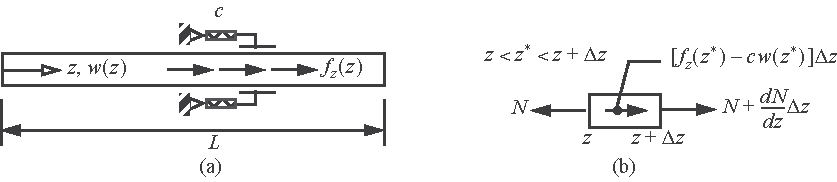
\includegraphics{Figure_17-1.pdf}
}{\caption{(a) Elastic bar subject to axial loading. (b) Free body of a segment of length $\Delta\textrm{z}$.\label{fig17.1}}}}


\section{Elastic bar subject to axial loads}\label{sec17.1}

The presentation in this section follows, in part, that given by Szabo and Babuska (1991). A prismatic bar of length \textit{L} and a cross-sectional area \textit{A} is shown in figure~\ref{fig17.1}(a). The bar is made of a homogeneous, linear elastic material whose modulus of elasticity is denoted by \textit{E} and its coefficient of thermal expansion by $\alpha$. Let the axial displacement function be denoted by $w(z)$ where $z$ is the axial coordinate and $0 \leq z \leq L$. Prescribed external loads consist of an axial distributed load with intensity $f_{z}(z)$ (F/L) and a change in temperature that is independent of the contour coordinate $s$ but a function of the axial coordinate $z$ (i.e., $\Delta T(s, z)=\tau_{0}(z)$). The bar is restrained by a distributed spring proportional to the axial displacement with an intensity given by $-c w(z)$ and $c \geq 0$ (F/L$^2$). A free body diagram of a segment of the bar is shown in figure~\ref{fig17.1}(b). The internal axial normal force is denoted by $N(z)$. Axial equilibrium of the segment as $\Delta z \rightarrow 0$ leads to the differential equation
\begin{align}\label{eq17.1}
-\left(\frac{d N}{d z}\right)+c w=f_{z}(z) \quad 0<z<L.
\end{align}
Hooke's law including the prescribed thermal force is $N+N_{T}=E A d w/d z$, where $N_{T}=E A \alpha \tau_{0}(z)$. Thus,
\begin{align}\label{eq17.2}
N=E A\left(\frac{d w}{d z}-\alpha \tau_{0}\right).
\end{align}
Substitute (\ref{eq17.2}) for the axial force in equilibrium equation (\ref{eq17.1}) to get the governing differential equation for axial displacement $w(z)$ as
\begin{align}\label{eq17.3}
-\frac{d}{d z}\left[E A\left(\frac{d w}{d z}-\alpha \tau_{0}\right)\right]+c w=f_{z}(z).
\end{align}
The boundary conditions at $z=0$ and $z=L$ are to prescribe either the displacement $w$ or the axial normal force \textit{N}. The displacement prescribed at the boundary is also called the essential boundary condition and the force prescribed at the boundary is called the natural boundary condition.

Multiply (\ref{eq17.3}) by an arbitrary axial displacement function $\bar{w}(z)$ and integrate:
\begin{align}\label{eq17.4}
-\int_{0}^{L}\left\{\frac{d}{d z}\left[E A\left(\frac{d w}{d z}-\alpha \tau_{0}\right)\right]-c w\right\} \bar{w}(z) d z=\int_{0}^{L} f_{z}(z) \bar{w}(z) d z.
\end{align}
Integrate the left-hand side of the previous equation by parts:
\begin{align}\label{eq17.5}
-\left\{\left.N \bar{w}\right|_{z=L}-\left.N \bar{w}\right|_{z=0}-\int_{0}^{L}\left\{\left[E A\left(\frac{d w}{d z}-\alpha \tau_{0}\right)\right] \frac{d \bar{w}}{d z}+c w \bar{w}\right\} d z\right\}=\int_{0}^{L} f_{z}(z) \bar{w}(z) d z.
\end{align}
Rearrange the terms in eq.~(\ref{eq17.5}) to get
\begin{align}\label{eq17.6}
\int_{0}^{L}\left\{E A \frac{d w}{d z} \frac{d \bar{w}}{d z}+c w \bar{w}\right\} d z=\int_{0}^{L} f_{z}(z) \bar{w}(z) d z+\left.N \bar{w}\right|_{z=L}-\left.N \bar{w}\right|_{z=0}+\int_{0}^{L}\left(E A \frac{d \bar{w}}{d z}\right) \alpha \tau_{0} d z.
\end{align}
If the governing boundary value problem for $w(z)$ (\ref{eq17.3}) is satisfied, then (\ref{eq17.6}) is also satisfied for any $\bar{w}(z)$ for which the operations in (\ref{eq17.6}) are defined. Note that in (\ref{eq17.6}) the highest derivative of the displacement is $d w/d z$, whereas the highest derivative in the differential equation (\ref{eq17.3}) is $\frac{d^{2} w}{d z^{2}}$. Integration by parts results in a derivative of one less in $w(z)$ than what occurs in the differential equation. Equation (\ref{eq17.6}) is called the \textbf{weak form} of the differential equation (\ref{eq17.3}).

\enlargethispage{-1\baselineskip}

In the finite element method the function $w(z)$ is called a \textbf{trial function}. The function $\bar{w}(z)$ is called a \textbf{test function} or a \textbf{virtual displacement}, and $d \bar{w}/d z$ is the virtual strain. Function $\bar{w}(z)$ is called a virtual displacement because it is not the actual physical displacement, but merely a hypothetical, admissible displacement. Each term in (\ref{eq17.6}) represents virtual work, that is, the work done by the internal action $E A d w/ d z$ through the virtual strain, work done by the distributed spring through the virtual displacement, work done by the prescribed distributed load and boundary forces through the virtual displacement, and the work of the virtual thermal force $E A d \bar{w}/d z$ due to the prescribed thermal strain $\alpha \tau_{0}$. Define
\begin{gather}
B[w, \bar{w}] \equiv \int_{0}^{L}\left\{E A \frac{d w}{d z} \frac{d \bar{w}}{d z}+c w \bar{w}\right\} dz, \textrm{ and}\label{eq17.7}\\
F[\bar{w}]\equiv \int_{0}^{L} f_{z}(z) \bar{w}(z) d z+\left.N \bar{w}\right|_{z=L}-\left.N \bar{w}\right|_{z=0}+\int_{0}^{L}\left(E A \frac{d \bar{w}}{d z}\right) \alpha \tau_{0} d z. \label{eq17.8}
\end{gather}
The bilinear form $B[w, \bar{w}]$ associates a real number with any two functions $w(z)$ and $\bar{w}(z)$, and the linear form $F[\bar{w}]$ associates a real number for any function $\bar{w}(z)$. The bilinear form $B[w, \bar{w}]$ represents the internal virtual work and the linear form $F[\bar{w}]$ represents the external virtual work. Let $U[w]$ denote the portion of the strain energy due to mechanical strain\footnote{Refer to eq. (\ref{eq5.81}) on page~\pageref{eq5.81}.} and that from the distributed spring. The expression for the strain energy is
\begin{align}\label{eq17.9}
U[w]=\frac{1}{2} \int_{0}^{L}\left\{E A\left(\frac{d w}{d z}\right)^{2}+c w^{2}\right\} d z=\frac{1}{2} B[w, w].
\end{align}
All continuous functions $w(z)$ defined on the open interval $\Omega \equiv\{z \mid 0<z<L\}$ have a finite strain energy $0 \leq U<\infty$, and $U=0$ only if $w(z)=0$ on $\Omega$. The conditions that restrict the set of all continuous functions having a finite strain energy are called displacement, kinematic, and essential boundary conditions. For example, if it is prescribed that the trial function $w(0)=q_{1}$ where $q_{1}$ has a numerical value, and the total displacement at $z$ = 0 is $w(0)+\bar{w}(0)=q_{1}$, then the virtual displacement $\bar{w}(0)=0$. The external virtual work for $\bar{w}(0)=0$ reduces to
\begin{align}\label{eq17.10}
F[\bar{w}]=\int_{0}^{L} f_{z}(z) \bar{w}(z) d z+\left.N \bar{w}\right|_{z=L}+\int_{0}^{L}\left(E A \frac{d \bar{w}}{d z}\right) \alpha \tau_{0} d z.
\end{align}
For displacement prescribed boundary conditions the virtual displacement must vanish at the boundaries. Kinematically admissible trial functions $w(z)$ are continuous, single valued, and equal to the prescribed displacement boundary conditions.

The \textbf{principle of virtual work} is to find a kinematically admissible displacement function $w(z)$ such that
\begin{align}
B[w, \bar{w}]=F[\bar{w}] \quad \text { for all kinematically admissible } \bar{w}(z). \label{eq17.11}
\end{align}
The principle of virtual work (\ref{eq17.11}) is a statement of equilibrium for the linear elastic bar, and it depends on the boundary conditions. The trial function $w(z)$ is selected to satisfy displacement boundary conditions, if any, on the closed domain $\Omega=\{z \mid 0 \leq z \leq L\}$. In the applications of the principle of virtual work it is not practical to consider an infinite number of kinematically admissible test functions. Instead, a subset of kinematically admissible functions is assumed. For example, polynomials in $z$ are often selected because they are easy to differentiate and integrate. Consider an approximate polynomial for the trial function $w(z)$ and a similar polynomial for the test function $\bar{w}(z)$ by selecting
\begin{align}\label{eq17.12}
w(z)=a_{1}+a_{2} z+a_{3} z^{2} \textrm{ and } \bar{w}(z)=b_{1}+b_{2} z+b_{3} z^{2}.
\end{align}
Unknown coefficients $a_{\textrm{i}}$ in the trial\enlargethispage{-1\baselineskip} function are determined from the principle of virtual work for every choice of the coefficients $b_{\textrm{i}}$, $i= 1$, 2, 3, in the test function. Coefficients $b_{\textrm{i}}$ are independent of the coefficients $a_{\textrm{i}}$ in the trial function.

\clearpage

\begin{example}[An approximate solution by the principle of virtual work]\label{ex17.1}Dimensional and material data for the bar shown in figure~\ref{fig17.1} are $L= 500$\,mm, $A= 400$\,mm$^{2}$, $E= 70{,}000$\,N/mm$^{2}$, $\alpha=23 . \times 10^{-6} /\left({ }^{\circ} \mathrm{C}\right)$, and $c=5 \times 10^{3}\,\mathrm{N}/\mathrm{mm}^{2}$. Uniform external loads are prescribed as $f_{z}(z)=0$ and a prescribed change in temperature $\tau_{0}(z)=40^{\circ} \mathrm{C}$ for $0<z<L$. Boundary conditions are $w(0)=q_{1}=-0.20\,\mathrm{mm}$ and $N(L)=F_{L}=-40{,}000\,\mathrm{N}$. Assume the trial and test functions for the displacements as
\begin{equation}
w(z)=q_{1}+a_{1} z \textrm{ and } \bar{w}(z)=b_{1} z. \label{eq17.1.a}\tag{a}
\end{equation}
Note that the trial function $w(z)$ satisfies the prescribed displacement boundary condition at $z=0$, and that the test function, or virtual displacement function, $\bar{w}(z)$ vanishes at $z=0$. The internal virtual work (\ref{eq17.7}) is
\begin{equation}
B[w, \bar{w}]=\int_{0}^{L}\left\{E A\left(a_{1}\right)\left(b_{1}\right)+c\left(q_{1}+a_{1} z\right)\left(b_{1} z\right)\right\} d z=b_{1}\left[\left(E A L+c L^{3}/3\right) a_{1}+\left(c L^{2}/2\right) q_{1}\right], \label{eq17.1.b}\tag{b}
\end{equation}
The external virtual work (\ref{eq17.8}) is
\begin{equation}
F[\bar{w}]=N(L)(\bar{w}(L))+\int_{0}^{L}\left(E A \frac{d \bar{w}}{d z}\right) \alpha \tau_{0} d z=b_{1}\left[L F_{L}+E A L \alpha \tau_{0}\right]. \label{eq17.1.c}\tag{c}
\end{equation}
The principle of virtual work (\ref{eq17.11}) for the assumed displacement functions is
\begin{equation}
b_{1}\left[\left(E A L+c L^{3}/3\right) a_{1}+\left(c L^{2}/2\right) q_{1}\right]=b_{1}\left[L F_{L}+E A L \alpha \tau_{0}\right] \quad \forall b_{1} \neq 0. \label{eq17.1.d}\tag{d}
\end{equation}
Hence, the equation to determine coefficient $a_1$ is
\begin{equation}
\left(E A L+\left(c L^{3}\right)/3\right) a_{1}+\left(c L^{2}/2\right) q_{1}=L F_{L}+E A L \alpha \tau_{0}. \label{eq17.1.e}\tag{e}
\end{equation}
Solve (\textbf{\ref{eq17.1.e}}) for $a_1$ to get
\begin{equation}
a_{1}=\frac{3\left(2 F L-c L q_{1}+2 E A \alpha \tau_{0}\right)}{2\left(3 E A+c L^{2}\right)}=530.195 \times 10^{-6}. \label{eq17.1.f}\tag{f}
\end{equation}
Note that $a_1$ is dimensionless. The following equations are the results for the axial displacement in eq. (\textbf{\ref{eq17.1.a}}), axial normal force in eq.~(\ref{eq17.2}), and the strain energy in eq.~(\ref{eq17.9}):
\begin{gather}
w(z)=-0.20+\left(530.195 \times 10^{-6}\right) z \quad 0 \leq z \leq 500\,\mathrm{mm}. \label{eq17.1.g}\tag{g} \\
N=E A\left[530.195 \times 10^{-6}-\left(23 . \times 10^{-6} /{ }^{\circ} \mathrm{C}\right) 40^{\circ} \mathrm{C}\right]=-10,914.5\,\mathrm{N} \quad 0 \leq z \leq 500\,\mathrm{mm}, \label{eq17.1.h}\tag{h} \\
U[w]=\frac{1}{2} \int_{0}^{L}\left\{E A\left(\frac{d w}{d z}\right)^{2}+c w^{2}\right\} d z=\frac{1}{2} \int_{0}^{L}\left\{E A\left(a_{1}\right)^{2}+c\left(q_{1}+a_{1} z\right)^{2}\right\} d z=14,975.3\,\textrm{N-mm}.  \label{eq17.1.i}\tag{i}
\end{gather}

The exact solution to the differential equation (\ref{eq17.3}) subject to the prescribed external loads and the prescribed boundary conditions is
\begin{equation}
w_{\mathrm{ex}}(z)=-0.20 \cosh \lambda z+0.199904 \sinh \lambda z \quad 0 \leq z \leq 500\,\mathrm{mm}, \label{eq17.1.j}\tag{j}
\end{equation}
where $\lambda=\sqrt{c /(E A)}=0.0133631\,\mathrm{mm}^{-1}$. The axial normal force and strain energy for the exact solution are
\begin{gather}
N_{\mathrm{ex}}=-25,760+74,797.2 \cosh \lambda z-74,833.1 \sinh \lambda z \quad 0 \leq z \leq 500\,\mathrm{mm}, \textrm{ and}\label{eq17.1.k}\tag{k} \\
U_{\mathrm{ex}}=7,754.26\,\textrm{N-mm}. \label{eq17.1.l}\tag{l}
\end{gather}
The strain energy of the approximate solution exceeds that of the exact solution. The error in the strain energy is
\begin{equation}
\frac{\left(U-U_{\mathrm{ex}}\right) 100}{U_{\mathrm{ex}}}=93.1 \%. \label{eq17.1.m}\tag{m}
\end{equation}
At $z=L$, $N_{\mathrm{ex}}=-40{,}000\,\mathrm{N}$ and for the approximate solution $N=-10{,}914.5\,\mathrm{N}$, an error of $-72.7$~percent. Graphs of the axial displacement distribution and axial force distribution are shown in figure~\ref{fig17.2} and figure~\ref{fig17.3}, respectively.

{\def\thefigure{17.2}
\processfigure{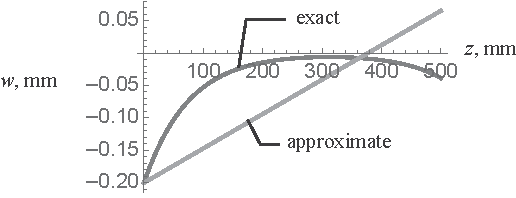
\includegraphics{Figure_17-2.pdf}
}{\caption{Axial displacement distribution for example~\ref{ex17.1}. The exact solution is\break compared to the approximate solution by the principle of virtual work.\label{fig17.2}}}}


{\def\thefigure{17.3}
\processfigure{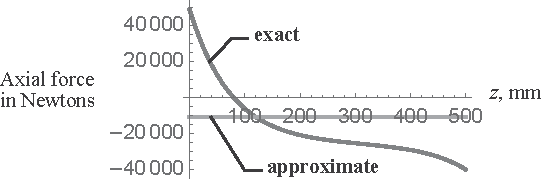
\includegraphics{Figure_17-3.pdf}
}{\caption{Axial normal force distribution in Newtons for example~\ref{ex17.1}. The exact solution compared to the approximate solution.\label{fig17.3}}}}


The displacement and axial force in the approximate solution do not compare well with the exact solution. Including polynomial terms of higher degree for the trial function and test functions (\textbf{\ref{eq17.1.a}}) results in improved approximate solutions. Rather than selecting polynomials of higher degree in the principle of virtual work, consider a finite element approximation using piecewise, linear polynomials as is discussed next in article~\ref{sec17.2}.
\end{example}

\vspace*{-1pc}

\section{Finite elements in one dimension}\label{sec17.2}

As stated in eq.~(\textbf{\ref{eq17.11}}) the principle of virtual work applies over the whole domain $\Omega$ of the bar. However, the principle of virtual work can also be applied to subdomains of the bar. In the finite element method we partition $\Omega$ into subdomains called finite elements. Partitions are called meshes, and finite element meshes are characterized by the selection of nodal points. Consider the mesh
\begin{align}\label{eq17.13}
0=z_{1}<z_{2}<z_{3}<\ldots<z_{M}<z_{M+1}=L,
\end{align}
where \textit{M} denotes the number of elements and $M+1$ is the number of nodes. The kth element is denoted by
\begin{align}\label{eq17.14}
\Omega_{k} \equiv\left\{z \mid z_{k} \leq z \leq z_{k+1}\right\} \quad k=1,2, \ldots, M.
\end{align}

\vspace*{-1pc}\pagebreak

\noindent Each element is mapped onto a standard element denoted by
\begin{align}\label{eq17.15}
\Omega_{\mathrm{st}} \equiv\{\zeta \mid-1<\zeta<1\}.
\end{align}
The standard element is mapped onto the kth element by
\begin{align}\label{eq17.16}
z=\eta_{1}(\zeta) z_{k}+\eta_{2}(\zeta) z_{k+1}, \textrm{ where } \eta_{1}(\zeta)=(1-\zeta)/2 \textrm{ and } \eta_{2}(\zeta)=(1+\zeta)/2
\end{align}
The inverse mapping is
\begin{align}\label{eq17.17}
\zeta=\frac{2 z-z_{z}-z_{k+1}}{z_{k+1}-z_{k}}=\frac{2 z-z_{z}-z_{k+1}}{h_{k}} \quad z \in \Omega_{k}.
\end{align}
The length of the element is denoted by $h_{k}$ where $h_{k}=z_{k+1}-z_{k}$. Functions $\eta_{i}(\zeta)$, $i=1$, 2, are called \textbf{shape functions} or \textbf{interpolation functions,} which have the properties
\begin{equation}
\eta_{1}(-1)=1 \quad \eta_{1}(1)=0 \quad \eta_{2}(-1)=0 \quad \eta_{1}(1)=1. \label{eq17.18}
\end{equation}

\vspace*{-1pc}

Kinematic admissibility requires the displacement function $w(z)$ to be continuous between elements and within an element. Continuity insures the derivative of the displacement is a square integrable function on $\Omega$ so that the strain energy (\ref{eq17.9}) is finite. The displacement in the kth element is denoted by $w^{(k)}(z)$, $z \in \Omega_{k}$. Let the displacements at the nodes $z_{k}$ and $z_{k+1}$ be denoted by $w^{(k)}\left(z_{k}\right)=q_{k}$ and $w^{(k)}\left(z_{k+1}\right)=q_{k+1}$, respectively. A linear polynomial in the axial coordinate with two coefficients is sufficient to interpolate the displacement at the two nodes, and it meets the continuity requirement within the element. The simple choice is to use the same linear interpolation functions for the displacement of the kth element as were used to interpolate coordinate $z \in \Omega_{k}$ (\textbf{\ref{eq17.16}}). Hence, the trial function for the axial displacement of the kth element is
\begin{equation}
w^{(k)}=\eta_{1}(\zeta) q_{k}+\eta_{2}(\zeta) q_{k+1} \quad \zeta \in \Omega_{\mathrm{st}}. \label{eq17.19}
\end{equation}
At node $z_{k+1}$ the displacement from the end of the kth element is $w^{(k)}\left(z_{k+1}\right)=\eta_{2}(1) q_{k+1}=q_{k+1}$, and the beginning displacement of the k+1 element is $w^{(k+1)}\left(z_{k+1}\right)=\eta_{1}(-1) q_{k+1}=q_{k+1}$. Thus, interelement continuity is satisfied. The virtual displacement for the kth element is assumed to be the same functional form as the trial function:
\begin{align}\label{eq17.20}
\bar{w}^{(k)}=\eta_{1}(\zeta) b_{k}+\eta_{2}(\zeta) b_{k+1} \quad \zeta \in \Omega_{\mathrm{st}},
\end{align}
where coefficients $b_{k}$ are independent of the trial function.

The axial strain in the kth element is $\varepsilon^{(k)}=\frac{d w^{(k)}}{d z}$. By the chain rule and the inverse mapping (\ref{eq17.17}) we transform the derivative with respect to $z$ to the derivative with respect to $\eta$ by
\begin{align}\label{eq17.21}
\frac{d \square}{d z}=\frac{d \square}{d \zeta} \frac{d \zeta}{d z}=\left(\frac{2}{h_{k}}\right) \frac{d \square}{d \zeta}.
\end{align}
Thus, the strain in the kth element is
\begin{align}\label{eq17.22}
\varepsilon^{(k)}=\frac{d w^{(k)}}{d z}=\left(\frac{d w^{(k)}}{d \zeta}\right)\left(\frac{d \zeta}{d z}\right)=\left(\frac{d \eta_{1}}{d \zeta} q_{k}+\frac{d \eta_{2}}{d \zeta} q_{k+1}\right)\left(\frac{2}{h_{k}}\right)=\left[-1/h_{k} 1/ h_{k}\right]\left[\begin{array}{@{}c@{}}q_{k} \\q_{k+1}\end{array}\right].
\end{align}
Note that the strain (\ref{eq17.22}) is spatially uniform in the element. The virtual strain $\bar{\varepsilon}^{(k)}$ is
\begin{align}\label{eq17.23}
\bar{\varepsilon}^{(k)}=\frac{d \bar{w}^{(k)}}{d z}=\left(\frac{d \eta_{1}}{d \zeta} b_{k}+\frac{d \eta_{2}}{d \zeta} b_{k+1}\right)\left(\frac{2}{h_{k}}\right)=
\left[\begin{array}{@{}ll@{}}
-1/h_{k} & \left.1/ h_{k}\right]\end{array}\right]\left[\begin{array}{@{}c@{}}
b_{k} \\b_{k+1}\end{array}\right].
\end{align}
The bilinear form (\ref{eq17.7}), or internal virtual work, for the kth element is
\begin{align}\label{eq17.24}
B_{k}[w^{(k)}, \bar{w}^{(k)}]=\int_{z_{k}}^{z_{k+1}} \bar{\varepsilon}^{(k)} E A \varepsilon^{(k)} d z+\int_{z_{k}}^{z_{k+1}} \bar{w}^{(k)} c w^{(k)} d z.
\end{align}
Substitute (\ref{eq17.22}) and (\ref{eq17.23}) for the strains, and (\ref{eq17.19}) and (\ref{eq17.20}) for the displacements, into the internal virtual work (\ref{eq17.24}) to get
\begin{align}\label{eq17.25}
B_{k}[w^{(k)}, \bar{w}^{(k)}]=\hspace*{-3pt}\int_{-1}^{1}\hspace*{-2pt}\left[b_{k} b_{k+1}\right]\left[\begin{array}{@{}c@{}}-1/h_{k} \\1/ h_{k}\end{array}\right] \textit{EA}\left[-1/h_{k} 1/h_{k}\right]\left[\begin{array}{@{}c@{}}q_{k} \\q_{k+1}\end{array}\right] \frac{h_{k}}{2} d \zeta+\hspace*{-3pt}\int_{-1}^{1}\hspace*{-1.5pt}\left[b_{k} b_{k+1}\right]\left[\begin{array}{@{}l@{}}\eta_{1} \\\eta_{2}\end{array}\right] \hspace*{-1pt}c\hspace*{-1pt}\left[\eta_{1} \eta_{2}\right]\left[\begin{array}{@{}c@{}}q_{k} \\q_{k+1}\end{array}\right] \frac{h_{k}}{2} d \zeta,
\end{align}
where $d z=\left(h_{k}/2\right) d \zeta$. Perform the matrix algebra in the latter equation to get
\begin{align}\label{eq17.26}
B_{k}[w^{(k)}, \bar{w}^{(k)}]=\left[b_{k} b_{k+1}\right]\left\{\begin{array}{@{}c@{}}1 \\\int \\-1\end{array}\left(\left[\begin{array}{@{}cc@{}}
\frac{E A}{h_{k}^{2}} & \frac{-E A}{h_{k}^{2}} \\[6pt]
\frac{-E A}{h_{k}^{2}} & \frac{E A}{h_{k}^{2}}
\end{array}\right] \frac{h_{k}}{2}+c\left[\begin{array}{@{}cc@{}}\eta_{1}^{2} & \eta_{1} \eta_{2} \\\eta_{1} \eta_{2} & \eta_{2}^{2}\end{array}\right] \frac{h_{k}}{2}\right) d \zeta\right\}\left[\begin{array}{@{}c@{}}q_{k} \\q_{k+1}\end{array}\right]=\left[\begin{array}{@{}c@{}}b_{k} b_{k+1}\end{array}\right]\left[K^{(k)}\right]\left[\begin{array}{@{}c@{}}q_{k} \\q_{k+1}\end{array}\right].
\end{align}
Perform the integration in eq.~(\ref{eq17.26}) to determine the element stiffness matrix $\left[K^{(k)}\right]$. The result is
\begin{align}\label{eq17.27}
\left[K^{(k)}\right]=\left[\begin{array}{@{}ll@{}}k_{11}^{(k)} & k_{12}^{k} \\[6pt]
k_{21}^{(k)} & k_{22}^{(k)}\end{array}\right]=\left[\begin{array}{@{}l@{}}\frac{E A}{h_{k}}+\frac{c h_{k}}{3} \frac{-E A}{h_{k}}+\frac{c h_{k}}{6} \\[6pt]
\frac{-E A}{h_{k}}+\frac{c h_{k}}{6} \frac{E A}{h_{k}}+\frac{c h_{k}}{3}\end{array}\right].
\end{align}
Take the virtual displacement equal to the trial displacement, or $\bar{w}(k)=w^{(k)}$, in (\ref{eq17.26}), which implies $b_{k}=q_{k}$ and $b_{k+1}=q_{k+1}$. Then, multiply the result by one-half to identify the strain energy in the kth element as
\begin{align}\label{eq17.28}
U^{(k)}=\frac{1}{2}\big(B_{k}\big[w^{(k)}, w^{(k)}\big]\big)=\frac{1}{2}\big[\begin{array}{@{}ll@{}}q_{k} & q_{k+1}\end{array}\big]\big[K^{(k)}\big]\left[\begin{array}{@{}c@{}}q_{k} \\q_{k+1}\end{array}\right].
\end{align}

\vspace*{-1pc}

The linear form (\ref{eq17.8}), or the external virtual work, for the kth element is
\begin{align}\label{eq17.29}
F_{k}\left[\bar{w}^{(k)}\right] \equiv \int_{z_{k}}^{z_{k+1}} f_{z}^{(k)}(z) \bar{w}^{(k)}(z) d z+\left.N^{(k)} \bar{w}^{(k)}\right|_{z=z_{k+1}}-\left.N^{(k)} \bar{w}^{(k)}\right|_{z=z_{k}}+\int_{z_{k}}^{z_{k+1}}(E A \bar{\varepsilon}^{(k)}) \alpha \tau_0^{(k)}(z) d z.
\end{align}
Substitute (\ref{eq17.20}) for the virtual displacement and (\ref{eq17.23}) for the virtual strain into the external virtual work (\ref{eq17.29}), followed by employing the mapping of $z \rightarrow \zeta$ (\ref{eq17.16}). The result is
\begin{align}
F_{k}\left[\bar{w}^{(k)}\right]&= \int_{-1}^{1}\hspace*{-3pt} f_{z}^{(k)}(\zeta)\left[\eta_{1}(\zeta) b_{k}+\eta_{2}(\zeta) b_{k+1}\right]\left(h_{k}/2\right) d \zeta\hspace*{-3pt}+\hspace*{-3pt}\int_{-1}^{1}\left[E A\left(b_{k}\left(\frac{-1}{h_{k}}\right)+b_{k+1}\left(\frac{1}{h_{k}}\right)\right)\right] \alpha \tau_{0}^{(k)}(\zeta)\left(\frac{h_{k}}{2}\right)  \nonumber\\
&\quad d \zeta+N^{(k)}\left(z_{k+1}\right) b_{k+1}-N^{(k)}\left(z_{k}\right) b_{k}, \label{eq17.30}
\end{align}
where
\begin{align}\label{eq17.31}
f_{z}^{\left({k}\right)}(\zeta)=f_{z}\left[\eta_{1}(\zeta) z_{k}+\eta_{2}(\zeta) z_{k+1}\right] \quad \tau_{0}^{(k)}(\zeta)=\tau_{0}\left[\eta_{1}(\zeta) z_{k}+\eta_{2}(\zeta) z_{k+1}\right] \quad \zeta \in \Omega_{\mathrm{st}}.
\end{align}

\vspace*{-1pc}\pagebreak

\noindent Arrange the terms in (\ref{eq17.30}) to
\begin{align}\label{eq17.32}
\begin{aligned}F_{k}\left[\bar{w}^{(k)}\right]&= b_{k}\left[\int_{-1}^{1} f_{z}^{(k)}(\zeta) \eta_{1}(\zeta) \frac{h_{k}}{2} d \zeta+\int_{-1}^{1} E A\left(\frac{-1}{2}\right) \alpha \tau_{0}^{(k)}(\zeta) d \zeta-N^{(k)}\left(z_{k}\right)\right] \\
&\quad + b_{k+1}\left[\int_{-1}^{1} f_{z}^{(k)}(\zeta) \eta_{2}(\zeta) \frac{h_{k}}{2} d \zeta+\left(\int_{-1}^{1} E A\left(\frac{1}{2}\right) \alpha \tau_{0}^{(k)}(\zeta) d \zeta\right)+N^{(k)}\left(z_{k+1}\right)\right]\end{aligned}.
\end{align}
The last expression for the external virtual work is written as
\begin{align}\label{eq17.33}
F_{k}\left[\bar{w}^{(k)}\right]=b_{k}\left[Q_{k}^{(k)}+F_{k}^{(k)}\right]+b_{k+1}\left[Q_{k+1}+F_{k+1}^{(k)}\right],
\end{align}
where we define
\begin{gather}
F_{k}^{(k)} \equiv \int_{-1}^{1} f_{z}^{(k)}(\zeta) \eta_{1}(\zeta) \frac{h_{k}}{2} d \zeta+\int_{-1}^{1} E A\left(\frac{-1}{2}\right) \alpha \tau_{0}^{(k)}(\zeta) d \zeta,\; Q_{k}^{(k)} \equiv-N^{(k)}\left(z_{k}\right) \label{eq17.34} \\
F_{k+1}^{(k)} \equiv \int_{-1}^{1} f_{z}^{(k)}(\zeta) \eta_{2}(\zeta) \frac{h_{k}}{2} d \zeta+\int_{-1}^{1} E A\left(\frac{1}{2}\right) \alpha \tau_{0}^{(k)}(\zeta) d \zeta, \textrm{ and } Q_{k+1} \equiv N^{(k)}\left(z_{k+1}\right) \label{eq17.35}
\end{gather}
The forces acting on the element separated from the nodes, and the forces acting on the nodes are depicted in figure~\ref{fig17.4}.

{\def\thefigure{17.4}
\processfigure{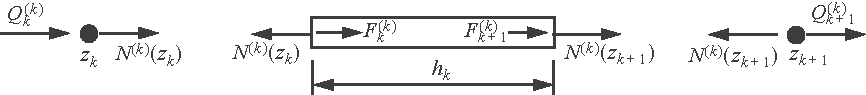
\includegraphics{Figure_17-4.pdf}
}{\caption{Forces acting on the bar and the nodes for element $\Omega_{\textrm{k}}$.\label{fig17.4}}}}



Finally, the external virtual work expression (\ref{eq17.33}) for the kth element is written as
\begin{gather}
F_{k}\left[\bar{w}^{(k)}\right]=\left\{b_{k}\right\}^{T}\left(\left\{Q^{(k)}\right\}+\left\{F^{(k)}\right\}\right), \textrm{ where}\label{eq17.36} \\
\left\{b_{k}\right\}=\left[\begin{array}{@{}c@{}}b_{k} \\b_{k+1}\end{array}\right], \left\{Q^{(k)}\right\}=\left[\begin{array}{@{}c@{}}Q_{k}^{(k)} \\[6pt] Q_{k+1}^{(k)}\end{array}\right], \textrm{ and } \left\{F^{(k)}\right\}=\left[\begin{array}{@{}l@{}}F_{k}^{(k)} \\[6pt] F_{k+1}^{(k)}\end{array}\right]. \label{eq17.37}
\end{gather}
The axial force in the kth element is
\begin{equation}
N^{(k)}=E A\left[\frac{2}{h_{k}} \frac{d w^{(k)}}{d \zeta}-\alpha \tau_{0}^{(k)}(\zeta)\right] \quad \zeta \in \Omega_{\mathrm{st}}. \label{eq17.38}
\end{equation}

\vspace*{-1pc}

The virtual work expressions for the \textit{M}-elements spanning $\Omega$ are
\begin{align}\label{eq17.39}
B[w, \bar{w}]=\sum_{k=1}^{M} B_{k}\left[w^{(k)}, \bar{w}^{(k)}\right] \quad F[\bar{w}]=\sum_{k=1}^{M} F_{k}\left[\bar{w}^{(k)}\right].
\end{align}

\vspace*{-1pc}\pagebreak

\noindent Consider in the summation of the external virtual work the terms from the k-1 element and the kth element. From (\ref{eq17.33}) these terms are
\begin{align}\label{eq17.40}
\hspace*{6pt}\underbrace{b_{k-1}\left[F_{k-1}^{(k-1)}+Q_{k-1}^{(k-1)}\right]+b_{k}\left[F_{k}^{(k-1)}+Q_{k}^{(k-1)}\right]}_{\text {element } \mathrm{k}-1}+\underbrace{b_{k}\left[F_{k}^{(k)}+Q_{k}^{(k)}\right]+b_{k+1}\left[F_{k+1}^{(k)}+Q_{k+1}^{(k)}\right]}_{\text {element k }}.
\end{align}
Combine the terms multiplying virtual displacement $b_{\textrm{k}}$ in eq.~(\ref{eq17.40}) to write the external virtual work as
\begin{align}\label{eq17.41}
F[\bar{w}]=\cdots+b_{k}\left[F_{k}^{(k-1)}+Q_{k}^{(k-1)}+F_{k}^{(k)}+Q_{k}^{(k)}\right]+\cdots.
\end{align}
At the common node $z_{\textrm{k}}$ let
\begin{equation}
Q_{k}=Q_{k}^{(k-1)}+Q_{k}^{(k)}=N^{(k-1)}\left(z_{k}\right)-N^{(k)}\left(z_{k}\right), \label{eq17.42}
\end{equation}
where $Q_{k}$ is the external axial force at node $z_{\textrm{k}}$. The definition of force $Q_{k}$ is based on equilibrium at node $z_{\textrm{k}}$ as shown by the free body diagram in figure~\ref{fig17.5}. Force $Q_{k}$ is prescribed if displacement $q_{\textrm{k}}$ is unknown, or it is an unknown reactive force if displacement $q_{\textrm{k}}$ is prescribed. At node $z_{\textrm{k}}$ the total external axial force consists of the contribution from the axial force $Q_{k}$ plus the distributed loading from the k-1 element and the kth element (i.e., $Q_{k}+F_{k}$, where $F_{k}=F_{k}^{(k-1)}+F_{k}^{(k)}$). A depiction of a finite element model with a mesh consisting of four nodes and three elements is shown in figure~\ref{fig17.6}.

{\def\thefigure{17.5}
\processfigure{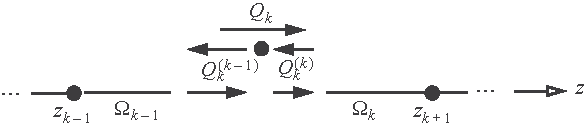
\includegraphics{Figure_17-5.pdf}
}{\caption{Free body diagram of node ${\textbf{\textit{z}}}_{\textbf{\textit{k}}}$.\label{fig17.5}}}}


{\def\thefigure{17.6}
\begin{figure}[!h]
\centerline{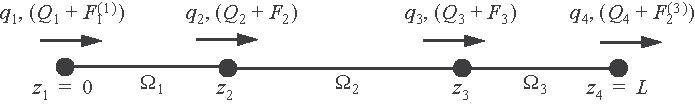
\includegraphics{Figure_17-6.pdf}}
\caption{A mesh consisting of four nodes and an assembly of three elements. Displacements and the
corresponding external forces are shown at each node.}\label{fig17.6}
\end{figure}}


If at node $z_{\textrm{k}}$ there is no prescribed externally applied point force, then we have the following relation from eq.~(\ref{eq17.42}):\vspace*{-12pt}
\begin{align}
Q_{k}=0=N^{(k-1)}\left(z_{k}\right)-N^{(k)}\left(z_{k}\right). \label{eq17.43}
\end{align}
Equation (\ref{eq17.43}) implies that the axial force is continuous at the node connecting the k-1 element to the kth element if $Q_{k}=0$. Displacement continuity at the common nodes is imposed in the finite element method. However, for the linear interpolation functions (\ref{eq17.20}) the axial force is, in general, discontinuous at the common nodes (i.e., $N^{(k-1)}\left(z_{k}\right)-N^{(k)}\left(z_{k}\right) \neq 0$). The jump in the axial force at common nodes decreases with mesh refinement as is illustrated in example~\ref{ex17.2} below.

\pagebreak

\begin{example}[Solution of example~\ref{ex17.1} using two finite elements] \label{ex17.2}
First consider a uniform mesh with $M=2$ using the interpolation functions (\ref{eq17.16}). The nodes are $z_{1}=0$, $z_{2}=L/2$, and $z_{3}=L$. The lengths of the elements are $h_{1}=h_{2}=L/2$. The total displacements for each element are
\begin{equation}
w^{(1)}(\zeta)=\eta_{1}(\zeta) q_{1}+\eta_{2}(\zeta) q_{2}, \textrm{ and } w^{(2)}(\zeta)=\eta_{1}(\zeta) q_{2}+\eta_{2}(\zeta) q_{3}. \label{eq17.2.a}\tag{a}
\end{equation}
The virtual displacements for each element are
\begin{equation}
\bar{w}^{(1)}(\zeta)=\eta_{2}(\zeta) b_{2} \textrm{ and } \bar{w}^{(2)}(\zeta)=\eta_{1}(\zeta) b_{2}+\eta_{2}(\zeta) b_{3}. \label{eq17.2.b}\tag{b}
\end{equation}
Note that virtual displacement in the first element at node one $\bar{w}^{(1)}(-1)=0$, since the displacement $q_1$ is prescribed at node one in the trial function.

The internal virtual work for elements one and two are
\begin{align}
B_{1}\left[w^{(1)}, \bar{w}^{(1)}\right] &=\left(\frac{2}{h_{1}}\right) \int_{-1}^{1} E A\left(\frac{d w^{(1)}}{d \zeta}\right)\left(\frac{d \bar{w}^{(1)}}{d \zeta}\right) d \zeta+\left(\frac{h_{1}}{2}\right) \int_{-1}^{1} c w^{(1)} \bar{w}^{(1)} d \zeta=b_{2}\left(k_{21}^{(1)} q_{1}+k_{22}^{(1)} q_{2}\right), \textrm{ and}\label{eq17.2.c}\tag{c}\\
B_{2}\left[w^{(2)}, \bar{w}^{(2)}\right] &=\left(\frac{2}{h_{2}}\right) \int_{-1}^{1} E A\left(\frac{d w^{\{2\}}}{d \zeta}\right)\left(\frac{d \bar{w}^{\{2\}}}{d \zeta}\right) d \zeta+\left(\frac{h_{2}}{2}\right) \int_{-1}^{1} c w^{(2)} \bar{w}^{(2)} d \zeta\nonumber\\
& =b_{2}\left[k_{11}^{(2)} q_{2}+k_{12}^{(2)} q_{3}\right]+b_{3}\left[k_{21}^{(2)} q_{2}+k_{22}^{(2)} q_{3}\right]. \label{eq17.2.d}\tag{d}
\end{align}
The element stiffness coefficients in eqs. (\textbf{\ref{eq17.2.c}}) and (\textbf{\ref{eq17.2.d}}) are given by eq.~(\ref{eq17.27}). For the assembly of the elements the total internal virtual work is
\begin{equation}
B=B_{1}\left[w^{(1)}, \bar{w}^{(1)}\right]+B_{2}\left[w^{(2)}, \bar{w}^{(2)}\right]=b_{2}\left[k_{21}^{(1)} q_{1}+\left(k_{22}^{(1)}+k_{11}^{(2)}\right) q_{2}+k_{12}^{(2)} q_{3}\right]+b_{3}\left[k_{21}^{(2)} q_{2}+k_{22^{\prime}} q_{3}\right]. \label{eq17.2.e}\tag{e}
\end{equation}
In matrix notation the internal virtual work for the assembly is
\begin{gather}
B=\left[\begin{array}{@{}ll@{}}b_{2} & b_{3}\end{array}\right]\left(\left[\begin{array}{@{}ll@{}}k_{22} & k_{23} \\k_{32} & k_{33}\end{array}\right]\left[\begin{array}{@{}l@{}}q_{2} \\q_{3}\end{array}\right]+\left[\begin{array}{@{}c@{}}k_{21}^{(1)} q_{1} \\0\end{array}\right]\right), \textrm{ where}\label{eq17.2.f}\tag{f}\\
k_{22}=k_{22}^{(1)}+k_{11}^{(2)} \quad k_{23}=k_{12}^{(2)} \quad k_{32}=k_{21}^{(2)} \quad k_{33}=k_{22}^{(2)} \quad k_{21}^{(1)}=-\frac{E A}{h_{1}}+\frac{c h_{1}}{6}. \label{eq17.2.g}\tag{g}
\end{gather}
Use the relation that $h_{1}=h_{2}=L/2$ to find that the stiffness matrix of the assembly is
\begin{equation}
\left[\begin{array}{@{}ll@{}}k_{22} & k_{23} \\k_{32} & k_{33}\end{array}\right]=\left[\begin{array}{@{}c@{}}\frac{4 E A}{L}+\frac{c L}{3} \mid \frac{-2 E A}{L}+\frac{c L}{12} \\[6pt]\frac{-2 E A}{L}+\frac{c L}{12} \mid \frac{2 E A}{L}+\frac{c L}{6}\end{array}\right]. \label{eq17.2.h}\tag{h}
\end{equation}
The external virtual work (\ref{eq17.33}) for the first element is
\begin{equation}
F\left[\bar{w}^{(1)}\right]=b_{2}\left(Q_{2}^{(1)}+F_{2}^{(1)}\right). \label{eq17.2.i}\tag{i}
\end{equation}
The external force from the change in temperature (\ref{eq17.35}) for the first element is
\begin{equation}
F_{2}^{(1)}=\int_{-1}^{1} E A\left(\frac{1}{2}\right) \alpha \tau_{0}^{(1)}(\zeta) d \zeta=E A \alpha \tau_{0}. \label{eq17.2.j}\tag{j}
\end{equation}
The external virtual work for the second element (\ref{eq17.33}) is
\begin{equation}
F_{2}\left[\bar{w}_{2}\right]=b_{2}\left(Q_2^{(2)}+F_2^{(2)}\right)+b_{3}\left(Q_{3}^{(2)}+F_{3}^{(2)}\right). \label{eq17.2.k}\tag{k}
\end{equation}
The external forces from the change in temperature for the second element are determined from eqs. (\ref{eq17.34}) and (\ref{eq17.35}):
\begin{equation}
F_{2}^{(2)}=\int_{-1}^{1} E A\left(\frac{-1}{2}\right) \alpha \tau_{0}^{2)}(\zeta) d \zeta=-E A \alpha \tau_{0}, \textrm{ and } F_{3}^{(2)}=\int_{-1}^{1} E A\left(\frac{1}{2}\right) \alpha \tau_0^{(2)}(\zeta) d \zeta=E A \alpha \tau_{0}. \label{eq17.2.l}\tag{l}
\end{equation}
The total external virtual work is the sum of the contributions from eqs. (\textbf{\ref{eq17.2.i}}) and (\textbf{\ref{eq17.2.k}}) is
\begin{equation}
F[\bar{w}]=F_{1}\left[\bar{w}^{(1)}\right]+F_{2}\left[\bar{w}_{2}\right]=b_{2}\left(Q_{2}^{(1)}+F_{2}^{(1)}+Q_{2}^{(2)}+F_{2}^{(2)}\right)+b_{3}\left(Q_{3}^{(2)}+F_{3}^{(2)}\right). \label{eq17.2.m}\tag{m}
\end{equation}
At node 2 there is no prescribed external force, so $Q_{2}=Q_{2}^{(1)}+Q_{2}^{(2)}=0$. Also at node 2 the sum of the thermal forces (\textbf{\ref{eq17.2.j}}) and (\textbf{\ref{eq17.2.l}}) is zero: that is, $F_{2}=F_{2}^{(1)}+F_{2}^{(2)}=E A \alpha \tau_{0}+\left(-E A \alpha \tau_{0}\right)=0$. Hence, the total external force at node 2 vanishes. At node 3 the prescribed force $Q_{3}=Q_{3}^{(2)}=F_{L}$, and the thermal force $F_{3}=F_{3}^{(2)}=E A \alpha \tau_{0}$. The total external virtual work is
\begin{equation}
F[\bar{w}]=\left[\begin{array}{@{}ll@{}}b_{2} & b_{3}\end{array}\right]\left[\begin{array}{@{}c@{}}0 \\F_{L}+E A \alpha \tau_{0}\end{array}\right]. \label{eq17.2.n}\tag{n}
\end{equation}

\vspace*{-1pc}

{\def\thefigure{17.7}
\processfigure[!b]{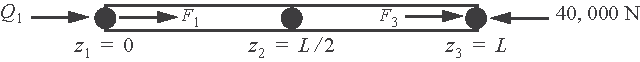
\includegraphics{Figure_17-7.pdf}
}{\caption{External forces acting on a two-element model.\label{fig17.7}}}}

Equate expressions (\textbf{\ref{eq17.2.f}}) and (\textbf{\ref{eq17.2.n}}) to get the principle of virtual work:
\begin{equation}
\left[\begin{array}{@{}ll@{}}b_{2} & b_{3}\end{array}\right]\left(\left[\begin{array}{@{}ll@{}}k_{22} & k_{23} \\k_{32} & k_{33}\end{array}\right]\left[\begin{array}{@{}l@{}}q_{2} \\q_{3}\end{array}\right]+\left[\begin{array}{@{}c@{}}k_{21}^{(1)} q_{1} \\[6pt]0\end{array}\right]\right)=\left[\begin{array}{@{}ll@{}}b_{2} & b_{3}\end{array}\right]\left[\begin{array}{@{}c@{}}0 \\[6pt]F_{L}+E A \alpha \tau_{0}\end{array}\right] \quad \boldsymbol{\forall}\left[\begin{array}{@{}ll@{}}b_{2} & b_{3}\end{array}\right] \neq 0_{1 X 2}. \label{eq17.2.o}\tag{o}
\end{equation}
It follows from eq. (\textbf{\ref{eq17.2.o}}) that the matrix equation to determine the displacements is
\begin{equation}
\left[\begin{array}{@{}ll@{}}k_{22} & k_{23} \\k_{32} & k_{33}\end{array}\right]\left[\begin{array}{@{}l@{}}q_{2} \\q_{3}\end{array}\right]=\left[\begin{array}{@{}c@{}}-k_{21}^{(1)} q_{1} \\[6pt] F_{L}+E A \alpha \tau_{0}\end{array}\right] \quad \text { where } \quad k_{21}^{(1)}=-\frac{2 E A}{L}+\frac{c L}{12}, \label{eq17.2.p}\tag{p}
\end{equation}
Note that the term involving displacement $q_1$ is known and so it is moved to the right-hand side of eq. (\textbf{\ref{eq17.2.p}}). Numerical evaluation of matrix equation (\textbf{\ref{eq17.2.p}}) is
\begin{equation}
\left[\begin{array}{@{}cc@{}}1.05733 \times 10^{6} & 96,333.3 \\96,333.3 & 528,667\end{array}\right]\left[\begin{array}{@{}l@{}}q_{2} \\q_{3}\end{array}\right]=\left[\begin{array}{@{}l@{}}19,266.7 \\-14,240\end{array}\right]. \label{eq17.2.q}\tag{q}
\end{equation}
The solution to matrix equation (\textbf{\ref{eq17.2.o}}) for the nodal displacements is $q_{2}=0.0210251\,\mathrm{mm}$ and $q_{3}=-0.0307669\,\mathrm{mm}$. The external forces acting on the bar modeled with two elements is shown in the free body diagram of figure~\ref{fig17.7}. Force $Q_{1}=Q_{1}^{(1)}$ is the reactive force at node~1 where the displacement is prescribed. The thermal force at node~1 $F_{1}=F_{1}^{(1)}=-E A \alpha \tau_{0}=-25{,}760\,\mathrm{N}$, which is evaluated from (\ref{eq17.34}). The thermal force at node~3 is $F_{3}=F_{3}^{(2)}=E A \alpha \tau_{0}=25{,}760\,\mathrm{N}$, which is evaluated from (\ref{eq17.35}). Then, axial equilibrium of the bar determines the reactive force $\textit{Q}_1 = 40{,}000$~N.



The trial functions for the displacements of the two elements are
\begin{gather}
w^{(1)}=-0.1(1-\zeta)+0.0105126(1+\zeta), \textrm{ and}\label{eq17.2.r}\tag{r}\\
w^{(2)}=0.0105126(1-\zeta)-0.0153834(1+\zeta). \label{eq17.2.s}\tag{s}
\end{gather}
The axial coordinate in element 1 is $z=\eta_{2}(\zeta)(250\,\mathrm{mm})$ and in element 2 it is $z=\eta_{1}(\zeta)(250\,\mathrm{mm})+\eta_{2}(\zeta)(500\,\mathrm{mm})$. The axial displacement is plotted with respect to $z$ from the exact solution given by eq. (\textbf{j}) in example~\ref{ex17.1} and from the finite element solution given by eqs. (\textbf{\ref{eq17.2.r}}) and (\textbf{\ref{eq17.2.s}}) in figure~\ref{fig17.8}. The finite element representation of the axial displacement is a piecewise linear polynomial, which is an improvement with respect to the virtual work result shown in figure~\ref{fig17.2}.

{\def\thefigure{17.8}
\processfigure{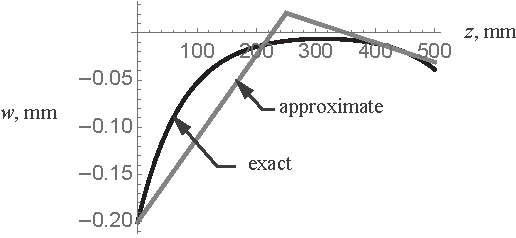
\includegraphics{Figure_17-8.pdf}
}{\caption{Axial displacement. Exact solution and an approximate solution using two finite elements.\label{fig17.8}}}}

{\def\thefigure{17.9}
\processfigure[!b]{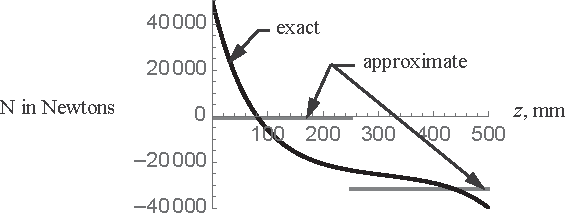
\includegraphics{Figure_17-9.pdf}
}{\caption{Axial force. Exact solution and an approximate solution using two finite elements.\label{fig17.9}}}}

The strain energy for the two element model is
\begin{equation}
U=\left(\frac{1}{2}\right) \sum_{k=1}^{M}\left[\frac{2}{h_{k}} \int_{-1}^{1} E A\left(\frac{d w^{(k)}}{d \zeta}\right)^{2} d \zeta+\frac{h_{k}}{2} \int_{-1}^{1} c\left(w^{(k)}\right)^{2} d \zeta\right]=10,589.9\,\textrm{N-mm}. \label{eq17.2.t}\tag{t}
\end{equation}
The error in the strain energy with respect to the exact value given by eq. (\textbf{\ref{eq17.2.l}}) in example~\ref{ex17.1} is
\begin{equation}
\frac{\left(U-U_{\mathrm{ex}}\right) 100}{U_{\mathrm{ex}}}=36.6 \%. \label{eq17.2.u}\tag{u}
\end{equation}
From (\ref{eq17.38}) the axial forces in each element are
\begin{equation}
N^{(1)}=E A\left[\frac{2}{h_{1}}\left(\frac{d w^{(1)}}{d \zeta}\right)-\alpha \tau_{0}\right]=-1,005.19\,\mathrm{N} \textrm{ and } N^{(2)}=E A\left[\frac{2}{h_{2}}\left(\frac{d w^{(2)}}{d \zeta}\right)-\alpha \tau_{0}\right]=-31,560.7\,\mathrm{N}. \label{eq17.2.v}\tag{v}
\end{equation}
The distributions of the axial force \textit{N} from the exact solution given by eq. (\textbf{\ref{eq17.2.k}}) in example~\ref{ex17.1} and the finite element solution (\textbf{\ref{eq17.2.v}}) are plotted in figure~\ref{fig17.9}. The finite element result for \textit{N} is piecewise constant, which is a improvement with respect to the virtual work result shown in figure~\ref{fig17.3}.
\end{example}


\subsection{Results from 4, 8, and 16 finite element solutions to example~\ref{ex17.1}}\label{sec17.2.1}

Improved numerical solutions are obtained by considering uniform meshes of four, eight, sixteen, etc., elements. As shown in figure~\ref{fig17.10}, the piecewise polynomial approximation for the axial displacement using eight uniform elements is, to the scale of the plot, very close to the exact solution. The axial force from the exact solution and from the finite element solution with eight uniform elements is shown in figure~\ref{fig17.11}. The piecewise constant axial force from the solution with eight elements is an improvement with respect to the two element model shown in figure~\ref{fig17.9}.

{\def\thefigure{17.10}
\processfigure{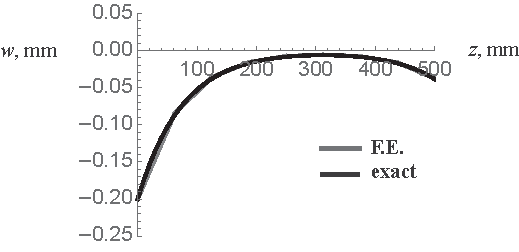
\includegraphics{Figure_17-10.pdf}
}{\caption{Axial displacement. Exact\break solution and an approximate solution\break using eight finite elements.\label{fig17.10}}}}


{\def\thefigure{17.11}
\processfigure[!h]{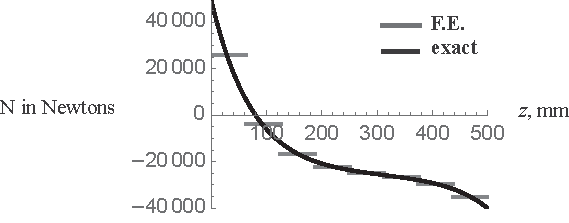
\includegraphics{Figure_17-11.pdf}}{\caption{Axial force. Exact~solu\-tion~and an approximate solution using eight finite elements.\label{fig17.11}}}}




The strain energy and the natural boundary condition at $z=L$ are used to measure the error in the finite element solutions with respect to the exact solution. Results for uniform meshes of one to sixteen elements are listed in table~\ref{tab17.1}. The data in the table demonstrates that the strain energy converges faster than the natural boundary condition to the exact solution as the number of elements is increased.

\begin{table}%17.1
\vspace*{-1pc}
\processtable{Errors in the strain energies and natural boundary conditions of example~\ref{ex17.1} as the number of element is increased. \label{tab17.1}}{%
\tabcolsep=12.5pt\begin{tabular}{@{\extracolsep\fill}lllll@{\extracolsep\fill}}
\toprule
\colhead{\textbf{M, number of}} & \colhead{\textbf{U, strain}} & \colhead{\textbf{Percentage error in the}} & \colhead{\textbf{N(L), Axial}} & \colhead{\textbf{Percentage error in the}} \\
\colhead{\textbf{uniform}} & \colhead{\textbf{energy,}} & \colhead{\textbf{strain energy}} & \colhead{\textbf{force in}} & \colhead{\textbf{axial force at}} \\
\colhead{\textbf{elements}} & \colhead{\textbf{N-mm}} & \colhead{\textbf{(U-Uex)100/Uex}} & \colhead{\textbf{Newtons}} & \colhead{\textbf{z~$=$~L [F$_{\textrm{L}}$ $-$ N(L)]100/F$_{\textrm{L}}$}} \\
\midrule
1$^{\textrm{a}}$ & 14,975.3 &  93.1$^{\textrm{b}}$ &  $-$10,914.5 &  72.7$^{\textrm{c}}$\\
2 &  10,589.9 &  36.6 &  $-$31,560.7 &  21.1\\
4 &  \phantom{0}8,551.95 &  10.3 &  $-$32,260.1 &  19.3\\
8 &  \phantom{0}7,961.15 &  \phantom{0}2.67 &  $-$35,260.1 &  11.8\\
16 &  \phantom{0}7,806.5 &  \phantom{0}0.674 &  $-$37,347.6 &  \phantom{0}6.63\\
\botrule
\end{tabular}}{a. From example~\ref{ex17.1}.\\
b. Uex~$=$~7,754.26 N-mm\\
c. FL~$= –40{,}000$ N}
\end{table}

\subsection{Convergence requirements}\label{sec17.2.2}

Heubner et~al. (1995, p. 85) list the following requirements for mathematical convergence of the finite element solution to the exact solution as an increasing number of smaller elements are used in the remeshng process.
\begin{itemize}
\item The elements must be made smaller in such a way that every point in the solution domain can always be within an element regardless of how small the element may be.
\item All previous meshes must be contained in the refined meshes.
\item The form of the interpolation functions must remain unchanged.
\end{itemize}
For example, the nodes in the mesh for $\textit{M} = 2$ are also contained in the mesh for $\textit{M} = 4$, nodes in the mesh for $\textit{M} = 4$ are also contained in the mesh for $\textit{M} = 8$, etc. The same linear interpolation functions (\ref{eq17.16}) are used in each discretization.

\pagebreak

\subsection{Apparent loadings from the 8- and 16-element solutions of example~\ref{ex17.1}}\label{sec17.2.3}

As illustrated in figure~\ref{fig17.11}, the axial force exhibits jumps at the nodes between neighboring elements. These jumps can be interpreted as a series of concentrated forces applied at the nodes, and these forces are called the \textbf{apparent loading} (Szabo and Babuska, p. 63). Let $\underline{Q}_{k}$ denote the apparent axial force at node $z_{k}$. From (\ref{eq17.42}), the apparent axial force in the positive $z$-direction at an interior node is
\begin{align}\label{eq17.44}
\underline{Q}_{k}=N^{(k-1)}\left(z_{k}\right)-N^{(k)}\left(z_{k}\right) \quad k=2,3,\,\ldots,\,M-1.
\end{align}
The forces at the nodes computed from the jump in the internal axial force are listed in table~\ref{tab17.2} for the 8-element model and for the 16-element model. Note that the sum of these forces $\underline{Q}_{k}$ vanishes in each model, which is a consequence of the principle work as a statement of equilibrium. At common interior nodes the force $\underline{Q}_{k}$ is smaller in the 16-element model than in the 8-element model.



\subsection{Adaptive mesh refinement beginning with the 8-element solution to example~\ref{ex17.1}}\label{sec17.2.4}

A uniform mesh may converge slowly to the exact solution with continued refinement. In practice, finite element simulations are performed on a structure where the exact solution is not known. For those structures whose exact solutions are unknown, the apparent loading from the finite element solution can be used in adaptive procedures to refine the mesh. Adaptive mesh refinement is based on assessing the relative error of the energy norm in each element between the original loading and the apparent loading (Szabo and Babuska, p. 63). The energy norm for a kinematically admissible function $w(z)$ is denoted by $\|w(z)\|$, and it is defined as the square root of the strain energy (\ref{eq17.9}) (i.e., $\|w\| \equiv \sqrt{U[w]}$). The mesh and shape functions of the original model are not changed in the second solution of the model subject to the apparent loading. Those elements exhibiting the largest discrepancy in the energy norm between the original loading and the apparent loading are subdivided to generate a new mesh. The new mesh will not be uniform, and is called quasi-uniform. The adaptive mesh procedure is repeated with respect to the new mesh. This repeated use of mesh refinement generates a sequence of meshes. An optimum mesh is achieved when the local error is distributed uniformly through the mesh (Heubner et al., p. 514).

Consider the eight-element model ($M= 8$) with nine nodes. The nine nodes in the uniform mesh are
\begin{align}\label{eq17.45}
\left\{z_{9}\right\}=\{0,1/8,1/4,3/8,1/2,5/8,3/4,7/8,1\} L.
\end{align}

\pagebreak\noindent Each element has the same length $h_{k}=z_{k+1}-z_{k}=L/8$, $k=1,2, \ldots, 8$. The dimensions of the restrained structural stiffness matrix $\left[K_{\alpha \alpha}\right]$ is 8X8. The displacement degrees of freedom and the corresponding forces are
\begin{equation}\label{eq17.46}
\hspace*{6pt}\left\{q_{\alpha}\right\}=\left[\begin{array}{@{}llll@{}}q_{2} & q_{3} & q_{4} & q_{5}, q_{6}, q_{7}, q_{8}, q_{9}\end{array}\right]^{T}, \textrm{ and } \left\{Q_{\alpha}\right\}=\left[Q_{2} Q_{3} Q_{4}, Q_{5}, Q_{6}, Q_{7}, Q_{8}, Q_{9}\right]^{T}.
\end{equation}
The nodal force vector for the original loading is\vspace*{-4pt}
\begin{align}\label{eq17.47}
\left\{Q_{\alpha}\right\}=\left[(8 E A/L-c L/48) q_{1}, 0,0,0,0,0,0,0, E A \alpha \tau_{0}+F_{L}\right]^{T}=[-79,183.3,0,0,0,0,0,0,0,-14240 .]^{T}.
\end{align}

\vspace*{-1.4pc}

\noindent The matrix equation $\left[K_{\alpha \alpha}\right]\left\{q_{\alpha}\right\}=\left\{Q_{\alpha}\right\}$ is solved numerically to determine the displacement vector $\left\{q_{\alpha}\right\}$. The axial displacement $w^{(k)}$ in each of the eight elements is computed from $\left\{q_{\alpha}\right\}$, followed by the computation of the energy norm in each element $\left\|w^{(k)}\right\|$, $k=1,2, \ldots, 8$.

For the apparent loading the nodal force vector from table~\ref{tab17.2} is
\begin{table}[!h]%17.2
\processtable{Apparent loading from the finite element solutions of example~\ref{ex17.1}. \label{tab17.2}}{%
\tabcolsep=21pt\begin{tabular}{@{\extracolsep\fill}lcd{7,3}d{2,0}d{3,4}@{\extracolsep\fill}}
\toprule
& \multicolumn{2}{c}{\colhead{\hspace*{-0.6pc}8 elements, 9 nodes}} & \multicolumn{2}{c}{\colhead{\hspace*{1pc}\textbf{16 elements, 17 nodes}}} \\[-6pt]
& \multicolumn{2}{c}{\hrulefill} & \multicolumn{2}{c@{}}{\hrulefill} \\
\colhead{\textit{z}} & \colhead{\textit{k}} & \multicolumn{1}{l}{\colhead{\textbf{$\underline{Q}_{k},\,\textit{N}$}}} & \multicolumn{1}{l}{\colhead{\textit{k}}} & \multicolumn{1}{l}{\colhead{\hspace*{2.1pt}\textbf{$Q_{k},\,\textit{N}$}}} \\
\midrule
0 & 1 & -25{,}950.  &  1  &  –35{,}743.3 \\
L/16  &   &  \multicolumn{1}{l}{{-}{-}{-}{-}{-}{-}{-}{-}{-}{-}{-}{-}{-}{-}}  &  2  &  21{,}139.1\\
L/8  &  2  &  29{,}906.9  &  3  &  13{,}889.4\\
3 L/16 &  &  \multicolumn{1}{l}{{-}{-}{-}{-}{-}{-}{-}{-}{-}{-}{-}{-}{-}{-}} &  4 &  9{,}134.26\\
L/4 &  3  & 12{,}697.5 &  5 &  6{,}019.91\\
5 L/16 &  &  \multicolumn{1}{l}{{-}{-}{-}{-}{-}{-}{-}{-}{-}{-}{-}{-}{-}{-}} &  6 &  3{,}986.67\\
3 L/8 &   4 &  5{,}510.35 &  7 &  2{,}669.461\\
7 L/16 & &   \multicolumn{1}{l}{{-}{-}{-}{-}{-}{-}{-}{-}{-}{-}{-}{-}{-}{-}} &  8 &  1{,}831.7\\
L/2 &  5 &  2{,}672.57 &  9 &  1{,}322.93\\
9 L/16 &  &  \multicolumn{1}{l}{{-}{-}{-}{-}{-}{-}{-}{-}{-}{-}{-}{-}{-}{-}} &  10 &  1{,}051.76\\
5 L/8 &  6 &  1{,}944.26 &  11 &  969.5\\
11 L/16 &  &  \multicolumn{1}{l}{{-}{-}{-}{-}{-}{-}{-}{-}{-}{-}{-}{-}{-}{-}} &  12 &  1{,}061.37\\
3 L/4 &  7  & 2{,}750.58 &  13 &  1{,}343.86\\
13 L/16 &  &  \multicolumn{1}{l}{{-}{-}{-}{-}{-}{-}{-}{-}{-}{-}{-}{-}{-}{-}} &  14 &  1{,}867.72\\
7 L/8 &  8  & 5{,}727.95 &  15 &  2{,}727.03\\
15 L/16 &  &  \multicolumn{1}{l}{{-}{-}{-}{-}{-}{-}{-}{-}{-}{-}{-}{-}{-}{-}} &  16 &  4{,}076.14\\
L~$=$~500 mm &  9 & -35{,}250.1 &  17 &  -37{,}347.6\\
\midrule
  & & \multicolumn{1}{c}{$\sum_{k=1}^{9}Q_{k}=0$}  &  & \multicolumn{1}{c}{$\sum_{k=1}^{17}Q_{k}=0$} \\
\botrule
\end{tabular}}{}
\vspace*{-18pt}
\end{table}
\begin{align}\label{eq17.48}
\left\{\underline{Q}_{\alpha}\right\}=[29,906.9\;12,679.5,510.35\;2,672.57\;1,944.26\;2,750.58\;5,727.95,\;-35,260.1].
\end{align}
\noindent Without changing the restrained structural stiffness matrix, the equation $\left[K_{\alpha \alpha}\right]\left\{\underline{q}_{\alpha}\right\}=\left\{\underline{Q}_{\alpha}\right\}$ is solved numerically for the displacement vector $\left\{\underline{q}_{\alpha}\right\}$. Note that $\left\{\underline{q}_{\alpha}\right\} \neq\left\{q_{\alpha}\right\}$. From the displacement vector $\left\{\underline{q}_{\alpha}\right\}$ the axial displacement in the kth element $\underline{w}^{(k)}$ is determined. The energy norm for the displacement in each element from the apparent loading is denoted by $\left\|\underline{w}^{(k)}\right\|$, $k=1,2, \ldots, 8$. Results for the energy norms from the original loading and apparent loading are listed in table~\ref{tab17.3}. Elements 1, 8, 2, 7, 3, 5, 4, and 6 have the largest to the smallest discrepancy in the energy norms.

\begin{table}[h]%17.3
\processtable{Element energy norms from the original and apparent loadings. \label{tab17.3}}{%
\tabcolsep=20pt\begin{tabular}{@{\extracolsep\fill}llll@{\extracolsep\fill}}
\toprule
 & \colhead{\textbf{Original loading}} & \colhead{\textbf{Apparent loading}} & \colhead{\textbf{Discrepancy}} \\
\colhead{\textbf{Element}}& \colhead{\textbf{$\left\|w_{k}\right\|$}} & \colhead{\textbf{$\left\|\underline{w}_{k}\right\|$}} & \colhead{\textbf{$\left\|w_{k}\right\|-\left\|\underline{w}_{k}\right\|$}} \\
\midrule
1 & 79.5058 &  120.577 &  $-$41.0708 \\
2 &  33.5923 &  \phantom{0}14.4801 &  \phantom{$-$}19.1122\\
3 &  14.1945 &  \phantom{0}12.1357 &  \phantom{$-$0}2.05885\\
4 &  \phantom{0}6.01526 &  \phantom{00}7.86369 &  \phantom{0}$-$1.84843\\
5 &  \phantom{0}2.76845 &  \phantom{00}4.69067 &  \phantom{0}$-$1.92222\\
6 &  \phantom{0}2.84924 &  \phantom{00}4.61159 &  \phantom{0}$-$1.76235\\
7 &  \phantom{0}6.26583 &  \phantom{0}12.0038 &  \phantom{0}$-$5.738\\
8 &  14.7925 &  \phantom{0}34.9373 &  $-$20.1448\\
\botrule
\end{tabular}}{}
\end{table}

Based on the data in table~\ref{tab17.3}, a quasi-uniform mesh is selected to increase the number of elements in the domain where the errors in energy norm are large. For example, a mesh of fifteen nodes and fourteen elements is illustrated below:
\begin{align}\label{eq17.49}
\left\{z_{15}\right\}=\{0,1/24,1/12,1/8,3/16,1/4,3/8,1/2,5/8,3/4,13/16,7/8,11/12,23/24,1\} L,
\end{align}
where the lengths of the elements are
\begin{align}\label{eq17.50}
\left\{h_{14}\right\}=\left\{\frac{L}{24}, \frac{L}{24}, \frac{L}{24}, \frac{L}{16}, \frac{L}{16}, \frac{L}{8}, \frac{L}{8}, \frac{L}{8}, \frac{L}{8}, \frac{L}{16}, \frac{L}{16}, \frac{L}{24}, \frac{L}{24}, \frac{L}{24}\right\}.
\end{align}
The mesh with nine nodes and the mesh with fifteen nodes are depicted in figure~\ref{fig17.12}. Nodes are clustered at the beginning and end of the domain of the 14-element model where discrepancies in the energy norm were the largest. A finite element analysis of this 14-element model resulted in a strain energy of the assembly of 7,788.23 N-mm, and a natural boundary condition $N(L)=-38{,}164.2\,\mathrm{N}$. Compared to the exact solution the percentage error in the strain energy is 0.438 percent, and the error in the natural boundary condition is 4.59 percent. Moreover, compared to the results from the 16-element model with a uniform mesh in table~\ref{tab17.1}, the 14-element model has a smaller error in the strain energy and a smaller error in the natural boundary condition.

{\def\thefigure{17.12}
\processfigure{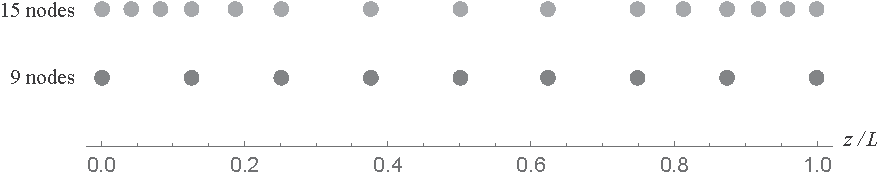
\includegraphics{Figure_17-12.pdf}
}{\caption{The nine-node uniform mesh and the fifteen-node quasi-uniform mesh.\label{fig17.12}}}}

\pagebreak

\section{A beam element including transverse shear deformation}\label{sec17.3}

The principle of virtual work is developed for a uniform beam of length \textit{L} that is symmetric about the \textit{y-z} plane as shown in figure~\ref{fig17.13}. It is subject to a lateral distributed load intensity $f_{y}(z)$ (F/L) and a change in temperature $\Delta T=\tau_{y}(z)y$, $0\leq z\leq L$, where $\tau_{y}(z) \left({ }^{\circ} \mathrm{C}/ \mathrm{L}\right)$ is the prescribed through the thickness temperature gradient. The\break $y$-direction displacement of the centroidal axis is denoted by $v(z)$ (L), and the rotation of the cross section about the $x$-axis is denoted by $\phi_{x}(z)$ (radians).

{\def\thefigure{17.13}
\begin{figure}[!h]
\centerline{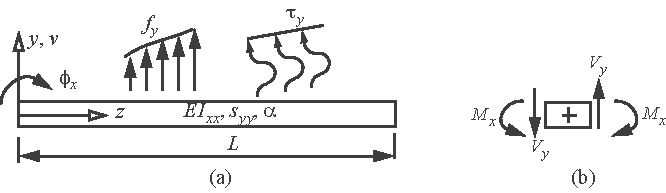
\includegraphics{Figure_17-13.pdf}}
\caption{(a) Symmetric beam subject to an external load and temperature gradient. (b) Definition for positive shear and moment.} \label{fig17.13}
\end{figure}}

The governing equations are as follows.
\begin{gather}
\textrm{equilibrium: } \frac{d V_{y}}{d z}+f_{y}(z)=0, \textrm{ and } \frac{d M_{x}}{d z}-V_{y}=0\quad 0<z<L. \label{eq17.51}\\
\textrm{Hooke's law: } V_{y}=s_{y y} \psi_{y}, \textrm{ and } M_{x}=E I_{x x}\left(\kappa-\alpha \tau_{y}\right). \label{eq17.52}\\
\textrm{strain-displacement: } \kappa=\frac{d \phi_{x}}{d z}, \textrm{ and } \psi_{y}=\frac{d v}{d z}+\phi_{x}. \label{eq17.53}
\end{gather}
The boundary conditions at $z=0$ and $z=L$ are to
\begin{equation}
\textrm{prescribe either } v \textrm{ or } V_{y}, \textrm{ and to prescribe either } \phi_{x} \textrm{ or } M_{x}\label{eq17.54}
\end{equation}
For a symmetric cross section the transverse shear stiffness $s_{y y}=1/c_{y y}$, where $c_{y y}$ (F$^{-1}$) is the transverse shear compliance. (Equations for the shear compliances are given by eq.~(\ref{eq5.62}) on page~\pageref{eq5.62} for an open cross-sectional contour and eq.~(\ref{eq5.85}) on page~\pageref{eq5.85} for a closed cross-sectional contour.)

Combine the equations associated with the shear force to get
\begin{align}\label{eq17.55}
\frac{d}{d z}\left[s_{y y}\left(\frac{d v}{d z}+\phi_{x}\right)\right]+f_{y}=0.
\end{align}
Multiply (\ref{eq17.55}) by the virtual displacement $\bar{v}(z)$ and integrate over the domain. Then integrate the result by parts to get
\begin{align}\label{eq17.56}
\left.\bar{v} V_{y}\right|_{0} ^{L}-\int_{0}^{L} s_{y y}\left(\frac{d v}{d z}+\phi_{x}\right)\left(\frac{d \bar{v}}{d z}\right) d z+\int_{0}^{L} f_{y} \bar{v} d z=0.
\end{align}
Combine the equations associated with the bending moment to get
\begin{align}\label{eq17.57}
\frac{d}{d z}\left[E I_{xx}\left(\frac{d \phi_{x}}{d z}-\alpha \tau_{y}\right)\right]-s_{y y}\left(\frac{d v}{d z}+\phi_{x}\right)=0.
\end{align}
Multiply (\ref{eq17.57}) by the virtual rotation $\bar{\phi}_{x}(z)$ and integrate over the domain. Then integrate the result by parts to find
\begin{align}\label{eq17.58}
\left.\bar{\phi}_{x} M_{x}\right|_{0} ^{L}-\int_{0}^{L}\left[E I_{x x}\left(\frac{d \phi_{x}}{d z}-\alpha \tau_{y}\right)\right]\left(\frac{d \bar{\phi}_{x}}{d z}\right) d z-\int_{0}^{L}\left[s_{y y}\left(\frac{d v}{d z}+\phi_{x}\right)\right] \bar{\phi}_{x} d z=0.
\end{align}
Equations (\ref{eq17.55}) and (\ref{eq17.57}) are coupled in the dependent variables $v(z)$ and $\phi_{x}(z)$, as are (\ref{eq17.56}) and (\ref{eq17.58}). To obtain the principle of virtual work for the two dependent variables we add (\ref{eq17.56}) and (\ref{eq17.58}) to find
\begin{align}\label{eq17.59}
\left.\bar{v} V_{y}\right|_{0} ^{L}+\left.\bar{\phi}_{x} M_{x}\right|_{0} ^{L}-\int_{0}^{L}\left[E I_{x x}\left(\frac{d \phi_{x}}{d z}-\alpha \tau_{y}\right)\right]\left(\frac{d \bar{\phi}_{x}}{d z}\right) d z-\int_{0}^{L} s_{y y}\left(\frac{d v}{d z}+\phi_{x}\right)\left(\frac{d \bar{v}}{d z}+\bar{\phi}_{x}\right) d z+\int_{0}^{L} f_{y} \bar{v} d z=0.
\end{align}
Rearrange the terms in eq.~(\ref{eq17.59}) to get the \textbf{weak form}
\begin{equation}
\int_{0}^{L}\left[E I_{x x}\left(\frac{d \phi_{x}}{d z}\right)\left(\frac{d \bar{\phi}_{x}}{d z}\right)+s_{y y} \psi_{y} \bar{\psi}_{y}\right] d z=\left.\bar{v} V_{y}\right|_{0} ^{L}+\left.\bar{\phi}_{x} M_{x}\right|_{0} ^{L}+\int_{0}^{L} f_{y} \bar{v} d z+\int_{0}^{L}\left(E I_{x x} \frac{d \bar{\phi}_{x}}{d z}\right) \alpha \tau_{y} d z, \label{eq17.60}
\end{equation}
where the virtual shear strain is
\begin{align}\label{eq17.61}
\bar{\psi}_{y}=\frac{d \bar{v}}{d z}+\bar{\phi}_{x}.
\end{align}

\vspace*{-1pc}

The \textbf{principle of virtual work} is determined from (\ref{eq17.60}) is written in the form
\begin{align}\label{eq17.62}
B\left[\phi_{x}, \bar{\phi}_{x}, v, \bar{v}\right]=F\left[\bar{\phi}_{x}, \bar{v}\right] \quad \text { for every kinematically admissible } \bar{\phi}_{x} \text { and } \bar{v}.
\end{align}
The internal virtual work is
\begin{align}\label{eq17.63}
B\left[\phi_{x}, \bar{\phi}_{x}, v, \bar{v}\right]=\int_{0}^{L}\left[E I_{x x}\left(\frac{d \phi_{x}}{d z}\right)\left(\frac{d \bar{\phi}_{x}}{d z}\right)+s_{y y} \psi_{y} \bar{\psi}_{y}\right] d z,
\end{align}
and the external virtual work is
\begin{align}\label{eq17.64}
F\left[\bar{\phi}_{x}, \bar{v}\right]=\left.\bar{v} V_{y}\right|_{0} ^{L}+\left.\bar{\phi}_{x} M_{x}\right|_{0} ^{L}+\int_{0}^{L} f_{y} \bar{v} d z+\int_{0}^{L}\left(E I_{x x} \frac{d \bar{\phi}_{x}}{d z}\right) \alpha \tau_{y} d z .
\end{align}
Equations (\ref{eq5.81}) and (\ref{eq5.82}) on page~\pageref{eq5.82} are the expressions for the strain energy. For the beam under consideration the strain energy from the mechanical strains is
\begin{align}\label{eq17.65}
U=\left(\frac{1}{2}\right) \int_{0}^{L}\left[E I_{x x}\left(\frac{d \phi_{x}}{d z}\right)^{2}+s_{y y}\left(\psi_{y}\right)^{2}\right] d z=\left(\frac{1}{2}\right) B\left[\phi_{x}, \phi_{x}, v, v\right].
\end{align}
The first term in the integral (\ref{eq17.65}) is the contribution of the bending to the strain energy, and the second term in the integral is the contribution of the transverse shear.


\subsection{Element displacement functions and strains}\label{sec17.3.1}

The kth element is denoted by $\Omega_{k} \equiv\left\{z \mid z_{k} \leq z \leq z_{k+1}\right\}$, where $z_{k}<z_{k+1}$. The standard element $\Omega_{\mathrm{st}} \equiv\{\zeta \mid-1<\zeta<1\}$ (\ref{eq17.15}) is mapped to the kth element by eq.~(\ref{eq17.16}), and the inverse mapping is given by eq.~(\ref{eq17.17}). The lateral displacement of the kth element is denoted by $v^{(k)}(z)$ and the rotation by $\phi_{X}^{(k)}(z)$ . Define the generalized nodal displacements as
\begin{align}\label{eq17.66}
v^{(k)}\left(z_{k}\right)=q_{2 k-1} \quad \phi_{x}^{(k)}\left(z_{k}\right)=q_{2 k} \quad v^{(k)}\left(z_{k+1}\right)=q_{2 k+1} \quad \phi_{x}^{(k)}\left(z_{k+1}\right)=q_{2 k+2}.
\end{align}

\begin{wrapfigure}[6]{r}{103pt}
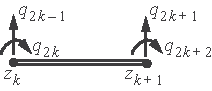
\includegraphics{Figure_17-14.pdf}
\caption{Generalized nodal displacements.\label{fig17.14}}
\end{wrapfigure}


See figure~\ref{fig17.14}. Admissible functions $v(z)$ and $\phi_{x}(z)$ must be continuous within an element and be continuous between elements. The following basis functions will be used for the beam element:
\begin{align}
\eta_{1}(\zeta) &=(1-\zeta)/2 \quad \eta_{2}(\zeta)=(1+\zeta)/2 \quad \eta_{3}(\zeta)=\left(\frac{1}{2} \sqrt{\frac{3}{2}}\right)\left(\zeta^{2}-1\right)\nonumber\\
\eta_{4}(\zeta)&=\left(\frac{1}{2} \sqrt{\frac{5}{2}}\right) \zeta\left(\zeta^{2}-1\right). \label{eq17.67}
\end{align}
The basis functions $\eta_{1}(\zeta)$ and $\eta_{2}(\zeta)$ are the \textbf{external shape functions} with the interpolation properties (\ref{eq17.18}). The basis functions $\eta_{3}(\zeta)$ and $\eta_{4}(\zeta)$ are called \textbf{internal shape functions}. The internal shape functions vanish at the nodes $\zeta=\mp 1$. The selection of the internal shape functions is based on Legendre polynomials. From Szabo and Babuska (1991, p. 38) the expressions for the internal shape function are
\begin{align}\label{eq17.68}
\eta_{j}(\zeta)=\frac{1}{\sqrt{2(2 j-1)}}\left[P_{j}(\zeta)-P_{j-1}(\zeta)\right] \quad j=3,4,
\end{align}
where $P_{j}(\zeta)$ is the Legendre polynomial of degree $j$ in $\zeta$.\footnote{$P_0 = 1$, $P_1=\zeta$, $P_2 = (3\zeta^{2}–1)/2$, $P_3= (5\zeta^{3}–3\zeta)/2$, $P_4 = (35\zeta^{4}–30\zeta^{2}+3)/8$.} Graphs of these basis functions are shown in figure~\ref{fig17.15}.

{\def\thefigure{17.15}
\processfigure{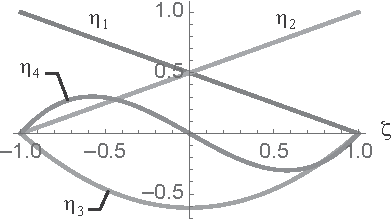
\includegraphics{Figure_17-15.pdf}
}{\caption{Graphs of the basis functions for the beam element.\label{fig17.15}}}}


Consider the strain $\kappa=d \phi_{x}/d z$ appearing in the bending moment (\ref{eq17.52}), and the rotation $\phi_{x}$ appearing in the transverse shear strain $\psi_{y}(\zeta)$ (\ref{eq17.53}). As discussed by Reddy (2019, p. 294), in order to avoid the numerical problem of ``shear locking'' in the thin beam limit where $\psi_{y} \rightarrow 0$, a consistent interpolation procedure is employed. That is, a consistent interpolation of the shear strain $\psi_{y}(\zeta)$ requires that the polynomial for the displacement $v(\zeta)$ be one degree greater in $\zeta$ than the polynomial for the rotation $\phi_{x}(\zeta)$. The beam element developed here is capable of representing a linear distribution of the bending moment $M_{x}(\zeta)$ and a constant shear force $V_{y}$. Then $d \phi_{x}/d z$ is linear in $\zeta$, which implies the rotation is quadratic in $\zeta$. It follows that displacement $v(\zeta)$ is cubic in $\zeta$. The trial functions for the kth element are
\begin{align}\label{eq17.69}
\begin{split}\phi_{x}^{(k)}(\zeta)&=\eta_{1}(\zeta) q_{2 k}+\eta_{2}(\zeta) q_{2 k+2}+\eta_{3}(\zeta) a_{2}^{(k)} \\
v^{(k)}(\zeta)&=\eta_{1}(\zeta) q_{2 k-1}+\eta_{2}(\zeta) q_{2 k+1}+\eta_{3}(\zeta) a_{1}^{(k)}+\eta_{4}(\zeta) a_{3}^{(k)}
\end{split}.
\end{align}
Internal degrees of freedom $a_{1}^{(k)}$ and $a_{3}^{(k)}$ are displacements with dimensions of length\textit{, }and $a_{2}^{(k)}$ is a rotation in radians. The internal degrees of freedom are not associated with a particular point in $\Omega_{\mathrm{st}}$. That is, the\vadjust{\pagebreak} beam element under consideration does not have internal nodes. Equation (\ref{eq17.69}) is written in the matrix notation as
\begin{align}\label{eq17.70}
\left[\begin{array}{@{}l@{}}\phi_{x}^{(k)} \\[3pt]v^{(k)}\end{array}\right]=\left[N_{q}(\zeta)\right]\left\{q^{(k)}\right\}+\left[N_{a}(\zeta)\right]\left\{a^{(k)}\right\},
\end{align}
where the 4X1 and the 3X1 vectors of generalized displacements are
\begin{align}\label{eq17.71}
\left\{q^{(k)}\right\}=\left[\begin{array}{@{}llll@{}}q_{2 k-1} & q_{2 k} & q_{2 k+1} & q_{2 k+2}\end{array}\right]^{T} \quad\left\{a^{(k)}\right\}=\left[\begin{array}{@{}lll@{}}a_{1}^{(k)} & a_{2}^{(k)} & a_{3}^{(k)}\end{array}\right]^{T}.
\end{align}
The shape function matrices are
\begin{align}\label{eq17.72}
\left[N_{q}(\zeta)\right]=\left[\begin{array}{@{}cccc@{}}0 & \eta_{1} & 0 & \eta_{2} \\\eta_{1} & 0 & \eta_{2} & 0\end{array}\right] \quad\left[N_{a}(\zeta)\right]=\left[\begin{array}{@{}ccc@{}}0 & \eta_{3} & 0 \\\eta_{3} & 0 & \eta_{4}\end{array}\right].
\end{align}
This beam element has seven degrees of freedom. The virtual rotation and displacement for the kth element have the same functional form as (\ref{eq17.70}) but with different coefficients:
\begin{align}\label{eq17.73}
\left[\begin{array}{@{}l@{}}\bar{\phi}_{x}^{(k)} \\[3pt]\bar{v}^{(k)}\end{array}\right]=\left[N_{q}(\zeta)\right]\left\{b^{(k)}\right\}+\left[N_{a}(\zeta)\right]\left\{c^{(k)}\right\},
\end{align}
where
\begin{align}\label{eq17.74}
\left\{b^{(k)}\right\}=\left[\begin{array}{@{}lllll@{}}b_{2 k-1} & b_{2 k} & b_{2 k+1} & b_{2 k+2}\end{array}\right]^{T} \quad\left\{c^{(k)}\right\}=\left[\begin{array}{@{}lll@{}}c_{1}^{(k)} & c_{2}^{(k)} & c 3_{3}^{(k)}\end{array}\right]^{T}.
\end{align}
Virtual degrees of freedom $\left[\begin{array}{@{}llll@{}}b_{2 k-1} & b_{2 k} & b_{2 k+1} & b_{2 k+2}\end{array}\right]$ are associated with the nodal displacements (external shape functions), and virtual degrees of freedom $\left[c_{1}^{(k)} c_{2}^{(k)} c_{3}^{(k)}\right]$ are associated with the internal shape functions. Elements of the virtual displacement vectors $\left\{b_{k}\right\}$ and $\left\{c^{(k)}\right\}$ are independent of the trial functions (\ref{eq17.69}).

Using the chain rule and the inverse mapping (\ref{eq17.17}), the strains for the kth element are
\begin{align}\label{eq17.75}
\frac{d \phi_{x}^{(k)}}{d z}=\left(\frac{2}{h_{k}}\right) \frac{d \phi_{x}^{(k)}}{d \zeta} \quad \psi_{y}^{(k)}=\left(\frac{2}{h_{k}}\right) \frac{d v^{(k)}}{d \zeta}+\phi_{x}^{(k)},
\end{align}
Substitute (\ref{eq17.70}) and (\ref{eq17.72}) into the expressions for the strains (\ref{eq17.75}) and write the strain-displacement relationship as
\begin{align}\label{eq17.76}
\left\{\varepsilon^{(k)}\right\}=\left[\begin{array}{@{}c@{}}\frac{d \phi_{x}^{(k)}}{d z} \\[3pt]\psi_{y}^{(k)}\end{array}\right]=\left[\begin{array}{@{}cccc@{}}0 & \frac{2}{h_{k}} \frac{d \eta_{1}}{d \zeta} & 0 & \frac{2}{h_{k}} \frac{d \eta_{2}}{d \zeta} \\[5pt]
\frac{2}{h_{k}} \frac{d \eta_{1}}{d \zeta} & \eta_{1} & \frac{2}{h_{k}} \frac{d \eta_{2}}{d \zeta} & \eta_{2}\end{array}\right]\left[\begin{array}{@{}c@{}}q_{2 k-1} \\[3pt]q_{2 k} \\[3pt]q_{2 k+1} \\[3pt]q_{2 k+2}\end{array}\right]+\left[\begin{array}{@{}ccc@{}}0 & \frac{2}{h_{k}} \frac{d \eta_{3}}{d \zeta} & 0 \\[3pt]
\frac{2}{h_{k}} \frac{d \eta_{3}}{d \zeta} & \eta_{3} & \frac{2}{h_{k}} \frac{d \eta_{4}}{d \zeta}\end{array}\right]\left[\begin{array}{@{}l@{}}a_{1}^{(k)} \\[5pt]a_{2}^{(k)} \\[5pt]a_{3}^{(k)}\end{array}\right].
\end{align}
In compact notation the strain-displacement relation (\ref{eq17.76}) is
\begin{align}\label{eq17.77}
\left\{\varepsilon^{(k)}\right\}=\left[\varepsilon_{q}(\zeta)\right]
\left\{q^{(k)}\right\}+\left[\varepsilon_{a}(\zeta)\right]\left\{a^{(k)}\right\},
\end{align}
where the strain-displacement matrices associated with the external shape functions and internal shape functions are
\begin{align}
\left[\varepsilon_{q}(\zeta)\right]=
\left[\begin{array}{@{}cccc@{}}
0 & \frac{-1}{h_{k}} & 0 & \frac{1}{h_{k}} \\[5pt]
\frac{-1}{h_{k}} & \frac{(1-\zeta)}{2} & \frac{1}{h_{k}} & \frac{(1+\zeta)}{2}
\end{array}\right] \quad\left[\varepsilon_{a}(\zeta)\right]=
\left[\begin{array}{@{}ccc@{}}
0 & \left(\frac{\sqrt{6}}{h_{k}} \zeta\right) & 0\\
\left(\frac{\sqrt{6}}{h_{k}} \zeta\right) & \left(\frac{1}{2} \sqrt{\frac{3}{2}}\left(\zeta^{2}-1\right)\right) & \left(\frac{1}{h_{k}} \sqrt{\frac{5}{2}}\left(3 \zeta^{2}-1\right)\right)\end{array}\right]. \label{eq17.78}
\end{align}
The virtual strains are polynomials of the same degree as strains (\ref{eq17.77}), but with independent coefficients:
\begin{align}\label{eq17.79}
\left\{\bar{\varepsilon}^{(k)}\right\}=\left[\begin{array}{@{}c@{}}\frac{d \bar{\phi}_{x}^{(k)}}{d z} \\[3pt]\bar{\psi}_{y}^{(k)}\end{array}\right]=\left[\varepsilon_{q}(\zeta)\right]\left\{b^{(k)}\right\}+\left[\varepsilon_{a}(\zeta)\right]\left\{c^{(k)}\right\}.
\end{align}

\vspace*{-0.6pc}

\subsection{Principle of virtual work for a typical element}\label{sec17.3.2}

The internal virtual work (\ref{eq17.63}) for the kth element in matrix notation is
\begin{align}\label{eq17.80}
B\left[\phi_{x}^{(k)}, \bar{\phi}_{x}^{(k)}, v^{(k)}, \bar{v}^{(k)}\right]=\frac{h_{k}}{2} \int_{-1}^{1}\left\{\bar{\varepsilon}^{(k)}\right\}^{T}[D]\left\{\varepsilon^{(k)}\right\} d \zeta,
\end{align}
where the material matrix is defined by\vspace*{-4pt}
\begin{align}\label{eq17.81}
[D] \equiv\left[\begin{array}{@{}cc@{}}E I_{x x} & 0 \\0 & s_{y y}\end{array}\right].
\end{align}
Substitute the strain-displacement matrices (\ref{eq17.77}) and (\ref{eq17.79}) into (\ref{eq17.80}) to get
\begin{align}
B\left[\phi_{x}^{(k)}, \bar{\phi}_{x}^{(k)}, v^{(k)}, \bar{v}^{(k)}\right] &=\frac{h_{k}}{2} \int_{-1}^{1}\left(\left\{b^{(k)}\right\}^{T}\left[\varepsilon_{q}(\zeta)\right]^{T}+\left\{c^{(k)}\right\}^{T}\left[\varepsilon_{a}(\zeta)\right]^{T}\right)\nonumber \\
&\quad\left([D]\left[\varepsilon_{q}(\zeta)\right]\left\{q^{(k)}\right\}  +[D]\left[\varepsilon_{a}(\zeta)\right]\left\{a^{(k)}\right\}\right) d \zeta. \label{eq17.82}
\end{align}
Perform the matrix multiplications in (\ref{eq17.82}) and arrange the result to
\begin{align}\label{eq17.83}
&\begin{array}{rl}B\left[\phi_{x}^{(k)}, \bar{\phi}_{x}^{(k)}, v^{(k)}, \bar{v}^{(k)}\right]\end{array}\nonumber\\
&\quad =
\left\{b^{(k)}\right\}^{T}\left\{\left(\frac{h_{k}}{2} \int^{1}_{-1}\left[\varepsilon_{q}(\zeta)\right]^{T}[D]\left[\varepsilon_{q}(\zeta)\right] d \zeta\right)\left\{q^{(k)}\right\}+\left(\frac{h_{k}}{2} \int^{1}_{-1}\left[\varepsilon_{q}(\zeta)\right]^{T}[D]\left[\varepsilon_{a}(\zeta)\right]\right\}\left\{a^{(k)}\right\}\right\} \nonumber\\
&\quad\quad\!\!+ \left. \left\{c^{(k)}\right\}^{T}\left\{\left(\frac{h_{k}^{1}}{2} \int^{1}_{-1}\left[\varepsilon_{a}(\zeta)\right]^{T}[D]\left[\varepsilon_{q}(\zeta)\right] d \zeta\right)\left\{q^{(k)}\right\}+\left(\frac{h_{k}}{2} \int^{1}_{-1}\left[\varepsilon_{a}(\zeta)\right]^{T}[D]\left[\varepsilon_{a}(\zeta)\right]\right\}\left\{a^{(k)}\right\}\right\}
\right\}.
\end{align}
The expression for the internal virtual work (\ref{eq17.83}) is written as
\begin{align}\label{eq17.84}
B\left[\phi_{x}^{(k)}, \bar{\phi}_{x}^{(k)}, v^{(k)}, \bar{v}^{(k)}\right]=\left\{b_{k}\right\}^{T}\left\{\left[K_{q q}\right]\left\{q^{(k)}\right\}+\left[K_{q a}\right]\left\{a^{(k)}\right\}\right\}+\left\{c^{(k)}\right\}^{T}\left\{\left[K_{a q}\right]\left\{q^{(k)}\right\}+\left[K_{a a}\right]\left\{a^{(k)}\right\}\right\},
\end{align}
where the stiffness matrices are defined by
\begin{gather}
\left[K_{q q}\right]=\frac{h_{k}}{2} \int_{-1}^{1}\left[\varepsilon_{q}(\zeta)\right]^{T}[D]\left[\varepsilon_{q}(\zeta)\right] d \zeta \quad\left[K_{q a}\right]=\frac{h_{k}}{2} \int_{-1}^{1}\left[\varepsilon_{q}(\zeta)\right]^{T}[D]\left[\varepsilon_{a}(\zeta)\right], \textrm{ and}\label{eq17.85}\\
\left[K_{a q}\right]=\frac{h_{k}}{2} \int_{-1}^{1}\left[\varepsilon_{a}(\zeta)\right]^{T}[D]\left[\varepsilon_{q}(\zeta)\right] d \zeta \quad\left[K_{a a}\right]=\frac{h_{k}}{2} \int_{-1}^{1}\left[\varepsilon_{a}(\zeta)\right]^{T}[D]\left[\varepsilon_{a}(\zeta)\right]. \label{eq17.86}
\end{gather}
Evaluate the stiffness matrices to find
\begin{gather}
\left[K_{q q}\right]=
\left[\begin{array}{@{}cccc@{}}
\frac{s_{y y}}{h_{k}} & \frac{-s_{y y}}{2} & \frac{-s_{y y}}{h_{k}} & \frac{-s_{y y}}{2} \\[5pt]
\frac{-s_{y y}}{2} & \frac{E I_{x x}}{h_{k}}+\frac{h_{k} s_{y y}}{3} & \frac{s_{y y}}{2} & \frac{-E I_{xx}}{h_{k}}+\frac{h_{k} s_{y y}}{6} \\[5pt]
\frac{-s_{y y}}{h_{k}} & \frac{s_{y y}}{2} & \frac{s_{y y}}{h_{k}} & \frac{s_{y y}}{2} \\[5pt]
\frac{-s_{y y}}{2} & \frac{-E I_{x x}}{h_{k}}+\frac{h_{k}  s_{y y}}{6} & \frac{s_{y y}}{2} & \frac{E I_{x x}}{h_{k}}+\frac{h_{k} s_{y y}}{3}\end{array}\right], \textrm{ and}\label{eq17.87}\\
\left[K_{q a}\right]
=\left[K_{a q}\right]^{T}
=\left[\begin{array}{@{\ }c;{2pt/2pt}c;{2pt/2pt}c@{\ }}
0 & \left(s_{y y}/\sqrt{6}\right) & 0 \\
\left(-s_{y y}/\sqrt{6}\right)   & \left(-h_{k} s_{y y} /(2 \sqrt{6})\right) & 0 \\
0 & \left(-s_{y y}/\sqrt{6}\right) & 0 \\
\left(s_{y y}/\sqrt{6}\right) & \left(-h_{k} s_{y y} /(2 \sqrt{6})\right) & 0\end{array}\right]
\quad
\left[K_{a a}\right]=
\left[\begin{array}{@{}cc;{2pt/2pt}c@{}}
\frac{2 s_{y y}}{h_{k}} & 0 & 0 \\
0 & \frac{E I_{x x}}{h_{k}}+\frac{h_{k} s_{y y}}{5} & \frac{s_{y y}}{\sqrt{15}} \\[5pt]
0 & \frac{s_{y y}}{\sqrt{15}} & \frac{2 s_{y y}}{h_{k}}\end{array}\right]. \label{eq17.88}
\end{gather}
Take $\left\{b^{(k)}\right\}=\left\{q^{(k)}\right\}$ and $\left\{c^{(k)}\right\}=\left\{a^{(k)}\right\}$ in (\ref{eq17.84}), and multiply the result by one-half, to find the strain energy in kth element as
\begin{align}\label{eq17.89}
U^{(k)}&=\frac{1}{2} B\left[\phi_{x}^{(k)}, \phi_{x}^{(k)}, v^{(k)}, v^{(k)}\right]\nonumber\\
&=\frac{1}{2}\left(\left\{q^{(k)}\right\}^{T}\left[K_{q q}\right]\left\{q^{(k)}\right\}+2\left\{q^{(k)}\right\}^{T}\left[K_{q q}\right]\left\{a^{(k)}\right\}+\left\{a^{(k)}\right\}^{T}\left[K_{a a}\right]\left\{a^{(k)}\right\}\right).
\end{align}
 From the mapping (\ref{eq17.16}), the distributed line load intensity and the thermal gradient are evaluated in the kth element as
\begin{equation}\label{eq17.90}
\begin{aligned}
&f_{y}\left[z_{k}(\zeta)\right]=f_{y}\left[z_{k} \eta_{1}(\zeta)+z_{k+1} \eta_{2}(\zeta)\right]=f_{y}^{(k)}(\zeta) \\
&\tau_{y}\left[z_{k}(\zeta)\right]=\tau_{y}\left[z_{k} \eta_{1}(\zeta)+z_{k+1} \eta_{2}(\zeta)\right]=\tau_{y}^{(k)}(\zeta)
\end{aligned}.
\end{equation}
The external virtual work (\ref{eq17.65}) for the kth element is
\begin{align}\label{eq17.91}
F\left[\bar{\phi}_{x}^{(k)}, \bar{v}^{(k)}\right]=\left.\bar{v}^{(k)} V_{y}^{(k)}\right|_{z_{k}} ^{z_{k+1}}+\left.\bar{\phi}_{x}^{(k)} M_{x}^{(k)}\right|_{z_{k}} ^{z_{k+1}}+\int_{-1}^{1} \bar{v}^{(k)} f_{y}^{(k)}(\zeta) \frac{h_{k}}{2} d \zeta+\int_{-1}^{1}\left(E I_{x x} \frac{d \bar{\phi}_{x}^{(k)}}{d \zeta} \frac{2}{h_{k}}\right) \alpha \tau_{y}^{(k)}(\zeta)\left(\frac{h_{k}}{2}\right) d \zeta.
\end{align}
The boundary terms for the kth element are expressed in the form
\begin{align}\label{eq17.92}
\left.\bar{v}^{(k)} V_{y}^{(k)}\right|_{z_{k}} ^{z_{k+1}}+\left.\bar{\phi}_{x}^{(k)} M_{x}^{(k)}\right|_{z_{k}} ^{z_{k+1}}=b_{2 k+1} Q_{2 k+1}^{(k)}+b_{2 k-1} Q_{2 k-1}^{(k)}+b_{2 k+2} Q_{2 k+2}^{(k)}+b_{2 k} Q_{2 k}^{(k)},
\end{align}
where generalized forces acting on the cross sections at $z= z_{\textrm{k}}$ and $z=z_{\textrm{k}+1}$ are defined by
\begin{align}\label{eq17.93}
Q_{2k-1}^{(k)} \equiv-V_{y}\left(z_{k}\right) \quad Q_{2k}(k) \equiv-M_{x}\left(z_{k}\right) \quad Q_{2 k+1}(k) \equiv V_{y}\left(z_{k+1}\right) \quad Q_{2 k+2}^{(k)} \equiv M_{x}\left(z_{k+1}\right). \hspace*{6pt}
\end{align}
The integral term with respect to the line load $f_{y}^{(k)}(\zeta)$ in (\ref{eq17.91}) expands to
\begin{align}\label{eq17.94}
\int_{1-1}^{1} \bar{v}^{(k)} f_{y}^{(k)}(\zeta) \frac{h_{k}}{2} d \zeta=\frac{h_{k}}{2}\left(\int_{-1}^{1}\left(b_{2 k-1} \eta_{1}+b_{2 k+1} \eta_{2}+c_{1}^{(k)} \eta_{3}+c_{3}^{(k)} \eta_{4}\right) f_{y}^{(k)}(\zeta) d \zeta\right).
\end{align}
The integral term with respect to the temperature gradient $\tau_{y}^{(k)}(\zeta)$ in (\ref{eq17.91}) expands to
\begin{align}\label{eq17.95}
\int_{-1}^{1}\left(E I_{x x} \frac{d \bar{\phi}_{x}^{(k)}}{d \zeta} \frac{2}{h_{k}}\right) \alpha \tau_{y}^{(k)}(\zeta)\left(\frac{h_{k}}{2}\right) d \zeta=\int_{-1}^{1} E I_{x x}\left(b_{2 k} \frac{d \eta_{1}}{d \zeta}+b_{2 k+2} \frac{d \eta_{2}}{d \zeta}+c_{2}^{(k)} \frac{d \eta_{3}}{d \zeta}\right) \alpha \tau_{y}^{(k)}(\zeta) d \zeta.
\end{align}
Combining (\ref{eq17.92}), (\ref{eq17.94}), and (\ref{eq17.95}), the external virtual work (\ref{eq17.91}) is written in the matrix form
\begin{align}\label{eq17.96}
F\left[\bar{\phi}_{x}^{(k)}, \bar{v}^{(k)}\right]=\left\{b^{(k)}\right\}^{T}\left(\left\{Q^{(k)}\right\}+\left\{F E^{(k)}\right\}\right)+\left\{c^{(k)}\right\}^{T}\left\{F I^{(k)}\right\},
\end{align}
where the generalized nodal force vector is denoted by $\left\{Q^{(k)}\right\}$, the generalized force vector associated with the external shape functions by $\left\{F E^{(k)}\right\}$, and the generalized force vector associated with the internal shape functions by $\left\{F I^{(k)}\right\}$. These vectors are
\begin{align}\label{eq17.97}
\left\{Q^{\{k\}}\right\}
\equiv
\left[\begin{array}{@{}c@{}}
Q_{2 k-1}^{(k)} \\[4pt]
Q_{2 k} \\[4pt]
Q_{2 k+1}^{k} \\[4pt]
Q_{2 k+2}^{(k)} \\[4pt]
\end{array}\right],
\left\{F E^{(k)}\right\}
=
\left[\begin{array}{@{}c@{}}
F E_{2 k-1}^{(k)} \\[4pt]
F E_{2 k}^{(k)} \\[4pt]
F E_{2 k+1}^{(k)} \\[4pt]
F E_{2 k+2}^{(k)}
\end{array}\right]
=
\left[
\begin{array}{@{}c@{}}
\frac{h_{k}}{2} \int^1_{-1}\eta_{1} f_{y}^{(k)} d\zeta \\[4pt]
\int^1_{-1} E I_{x x} \frac{d \eta_{1}}{d \zeta} \alpha \tau_{y}^{(k)} d \zeta \\[4pt]
\frac{h_{k}}{2} \int^1_{-1} \eta_{2} f_{y}^{(k)} d \zeta \\[4pt]
\int^1_{-1} E I_{x x} \frac{d \eta_{2}}{d \zeta} \alpha \tau_{y}^{(k)} d \zeta
\end{array}
\right]\!,
\left\{F I^{(k)}\right\}
=\left[\begin{array}{@{}c@{}}
F I_{1}^{(k)} \\[4pt]
F I_{2}^{(k)} \\[4pt]
F I_{3}^{(k)}
\end{array}\right]
=
\left[\begin{array}{@{}c@{}}
\frac{h_{k}}{2} \int^1_{-1} \eta_{3} f_{y}^{(k)} d \zeta \\[4pt]
\int^1_{-1} E I_{x x} \frac{d \eta_{3}}{d \zeta} \alpha \tau_{y}^{(k)} d \zeta\\[4pt]
\frac{h_{k}}{2} \int^1_{-1} \eta_{4} f_{y}^{(k)} d \zeta\end{array}\right].
\end{align}

Equate the internal virtual work (\ref{eq17.84}) to the external virtual work (\ref{eq17.96}) to get
\begin{align}\label{eq17.98}
&\left\{b^{(k)}\right\}^{T}\left(\left[K_{q q}\right]\left\{q^{(k)}\right\}+\left[K_{q a}\right]\left\{a^{\{k\}}\right\}\right)+\left\{c^{\{k\}}\right\}^{T}\left(\left[K_{a q}\right]\left\{q^{\{k\}}\right\}+\right. {\left.\left[K_{a a}\right]\left\{a^{(k)}\right\}\right)} \nonumber\\
&\quad =\left\{b^{(k)}\right\}^{T}\left(\left\{Q^{(k)}\right\}+\left\{F E^{(k)}\right\}\right)+\left\{c^{\{k\}}\right\}{ }^{T}\left\{F I^{(k)}\right\}.
\end{align}
The principle of virtual work leads to the governing matrix relations for the kth element:
\begin{gather}
\left[K_{q q}\right]\left\{q^{(k)}\right\}+\left[K_{q a}\right]\left\{a^{(k)}\right\}=\left\{Q^{(k)}\right\}+\{F E(k)\} \quad \boldsymbol{\forall}\left\{b^{(k)}\right\} \neq 0_{4 X 1}, \label{eq17.99} \\
\left[K_{a q}\right]\left\{q^{(k)}\right\}+\left[K_{a a}\right]\left\{a^{(k)}\right\}=\left\{F I^{(k)}\right\} \quad \boldsymbol{\forall}\left\{c^{(k)}\right\} \neq 0_{3 X 1}. \label{eq17.100}
\end{gather}



\subsection{Static condensation}\label{sec17.3.3}

The internal degrees of freedom $a_{1}^{(k)}$, $a_{2}^{(k)}$, and $a_{3}^{(k)}$ associated with the internal shape functions do not affect interelement continuity. To reduce the number of system equations to solve resulting from the assembly of elements, the internal degrees of freedom can be eliminated at the element level in the process called static condensation. Further, the assembly algorithm is simplified if only the nodal displacements, or external degrees of freedom are employed. The internal degrees of freedom are eliminated in terms of the nodal displacements $\left\{q^{(k)}\right\}$ and the generalized force vector $\left\{F I^{(k)}\right\}$ by solving (\ref{eq17.100}). Thus, from (\ref{eq17.100})
\begin{align}\label{eq17.101}
\left\{a^{(k)}\right\}=\left[K_{a a}\right]^{-1}\left\{F I^{(k)}\right\}-\left[K_{a a}\right]^{-1}\left[K_{a q}\right]\left\{q^{(k)}\right\}=\left[K_{a a}\right]^{-1}\left\{F I^{(k)}\right\}+\left[G_{a q}\right]\left\{q^{(k)}\right\},
\end{align}
where
\begin{align}\label{eq17.102}
\left[K_{a a}\right]^{-1}
=\left[\begin{array}{@{}ccc@{}}
\frac{h_{k}}{2 s_{y y}} & 0 & 0 \\[4pt]
0 & \frac{6 h_{k} \mu}{E I_{x x}} & \frac{-\sqrt{\frac{3}{5}} h_{k}^{2} \mu}{E I_{x x}} \\[4pt]
0 & \frac{-\sqrt{\frac{3}{5}} h_{k}^{2} \mu}{E I_{x x}} & \frac{30 E I_{x x} h_{k}+3 h_{k}^{3} s_{y y}}{60 E I_{x x} s_{y y}+5 h_{k}^{2} s_{y y}^{2}}\end{array}\right] \left[G_{a q}\right]
=\left[\begin{array}{@{}cccc@{}}
0 & \frac{h_{k}}{2 \sqrt{6}} & 0 & \frac{-h_{k}}{2 \sqrt{6}} \\[4pt]
\frac{-\sqrt{6} h_{k} s_{y y} \mu}{E I_{x x}} & \frac{\sqrt{\frac{3}{2}} h_{k}^{2} s_{y y} \mu}{E I_{x x}} & \frac{\sqrt{6} h_{k} s_{y y} \mu}{E I_{x x}} & \frac{\sqrt{\frac{3}{2}} h_{k}^{2} s_{y y} \mu}{E I_{x x}} \\[4pt]
\frac{h_{k}^{2} s_{y y} \mu}{\sqrt{10} E I_{x x}} & \frac{-h_{k}^{3} s_{y y} \mu}{2 \sqrt{10} E I_{x x}} & \frac{-h_{k}^{2} s_{y y} \mu}{\sqrt{10} E I_{x x}} & \frac{-h_{k}^{3} s_{y y} \mu}{2 \sqrt{10} E I_{x x}}\end{array}\right].
\end{align}
We define $\left[G_{aq}\right]$ as the Guyan matrix, because the method of static condensation was first proposed by Guyan (1965), and it was also introduced by Irons (1965). In eq.~(\ref{eq17.102}) we have introduced the dimensionless factor
\begin{align}\label{eq17.103}
\mu=\frac{E I_{x x}}{12 E I_{x x}+h_{k}^{2} s_{y y}}.
\end{align}
Substitute the displacement vector $\left\{a^{(k)}\right\}$ from (\ref{eq17.101}) into eq.~(\ref{eq17.99}) and write the final result as
\begin{align}\label{eq17.104}
\left[K^{(k)}\right]\left\{q^{(k)}\right\}=\left\{Q^{(k)}\right\}+\left\{F^{(k)}\right\},
\end{align}
where
\begin{align}\label{eq17.105}
\begin{gathered} {\left[K^{(k)}\right]=\left[K_{q q}\right]+\left[K_{q a}\right]\left[G_{a q}\right]} \\ \left\{F^{(k)}\right\}=\left\{F E^{(k)}\right\}-\left[K_{q a}\right]\left[K_{a a}\right]^{-1}\left\{F I^{(k)}\right\}=\left\{F E^{(k)}\right\}+\left[G_{a q}\right]^{T}\left\{F I^{(k)}\right\}\end{gathered}.
\end{align}
The 4X4 matrix $\left[K^{(k)}\right]$ is the condensed stiffness matrix for the kth element, and the 4X1 vector $\left\{F^{(k)}\right\}$ is the condensed generalized force vector for the kth element. The generalized forces acting on the beam element separated from the nodes, and the generalized forces acting on the nodes, are depicted in figure~\ref{fig17.16}.

{\def\thefigure{17.16}
\processfigure{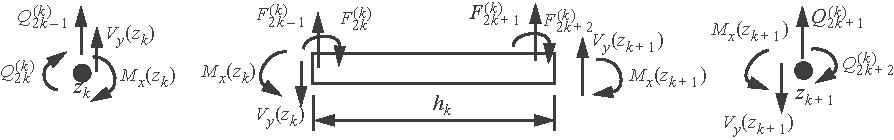
\includegraphics{Figure_17-16.pdf}
}{\caption{Generalized forces acting on the beam and the nodes for element $\Omega_{\textrm{k}}$.\label{fig17.16}}}}



The 4X4 condensed stiffness matrix is
\begin{align}\label{eq17.106}
\left[K^{(k)}\right]=\mu\left[\begin{array}{@{}cccc@{}}\frac{12 s_{y y}}{h_{k}} & -6 s_{y y} & \frac{-12 s_{y y}}{h_{k}} & -6 s_{y y} \\[4pt]-6 s_{y y} & \frac{12 E I_{x x}}{h_{k}}+4 h_{k} s_{y y} & 6 s_{y y} & \frac{-12 E I_{x x}}{h_{k}}+2 h_{k} s_{y y} \\[4pt]\frac{-12 s_{y y}}{h_{k}} & 6 s_{y y} & \frac{12 s_{y y}}{h_{k}} & 6 s_{y y} \\[4pt]-6 s_{y y} & \frac{-12 E I_{x x}}{h_{k}}+2 h_{k} s_{y y} & 6 s_{y y} & \frac{12 E I_{x x}}{h_{k}}+4 h_{k} s_{y y}\end{array}\right].
\end{align}


\subsection{Bending moment and shear force}\label{sec17.3.4}

Substitute vector $\left\{a^{(k)}\right\}$ from (\ref{eq17.101}) into the strain vector (\ref{eq17.77}) to get
\begin{align}\label{eq17.107}
\left\{\varepsilon^{(k)}\right\}=\left[\varepsilon_{q}(\zeta)\right]\left\{q^{(k)}\right\}+\left[\varepsilon_{a}(\zeta)\right]\left\{a^{(k)}\right\}=\left(\left[\varepsilon_{q}(\zeta)\right]+\left[\varepsilon_{a}\right]\left[G_{a q}\right]\right)\left\{q^{(k)}\right\}+\left[\varepsilon_{a}(\zeta)\right]\left[K_{a a}\right]^{-1}\left\{F I^{(k)}\right\}.
\end{align}
The bending moment and shear force are determined from the matrix relation
\begin{align}\label{eq17.108}
\left[\begin{array}{@{}c@{}}M_{x}^{(k)} \\V_{y}^{(k)}\end{array}\right]=[D]\left(\left\{\varepsilon^{(k)}\right\}-\left[\begin{array}{@{}c@{}}\alpha \tau_{y}^{(k)} \\0\end{array}\right]\right).
\end{align}
Substitute the strain (\ref{eq17.107}) into (\ref{eq17.108}) to find the matrix relation for the moment and shear:
\begin{align}\label{eq17.109}
\left[\begin{array}{@{}c@{}}M_{x}^{(k)} \\V_{y}^{(k)}\end{array}\right]=[D]\left(\left[\varepsilon_{q}(\zeta)\right]+\left[\varepsilon_{a}\right]\left[G_{a q}\right]\right)\left\{q^{(k)}\right\}+[D]\left(\left[\varepsilon_{a}(\zeta)\right]\left[K_{a a}\right]^{-1}\left\{F I^{(k)}\right\}-\left[\begin{array}{@{}c@{}}\alpha \tau_{y}^{(k)} \\0\end{array}\right]\right).
\end{align}
The previous equation is written as
\begin{align}\label{eq17.110}
\left[\begin{array}{@{}c@{}}M_{x}^{(k)} \\V_{y}^{(k)}\end{array}\right]=\left[S_{q}(\zeta)\right]\left[\begin{array}{@{}c@{}}q_{2 k-1} \\q_{2 k} \\q_{2 k+1} \\q_{2 k+2}\end{array}\right]+\left[S_{F}(\zeta)\right]\left[\begin{array}{@{}l@{}}F I_{1}^{(k)} \\F I_{2}^{(k)} \\F I_{3}^{(k)}\end{array}\right]-\left[\begin{array}{@{}c@{}}E I_{x x} \alpha \tau_{y}^{(k)}(\zeta) \\0\end{array}\right],
\end{align}
where the stress matrices are defined as
\begin{align}
\left[S_{q}(\zeta)\right]&=
\left[\begin{array}{@{}cccc@{}}
-6 s_{y y} \mu \zeta & \left(\frac{-E I_{x x}}{h_{k}}+3 h_{k} s_{y y} \mu \zeta\right) & 6 s_{y y} \mu \zeta & \left(\frac{E I_{x x}}{h_{k}}+3 h_{k} s_{y y} \mu \zeta\right) \\
\frac{-12 \mu s_{y y}}{h_{k}} & 6 s_{y y} \mu & \frac{12 \mu s_{y y}}{h_{k}} & 6 s_{y y} \mu
\end{array}\right], \textrm{ and}\label{eq17.111}\\
\left[S_{F}(\zeta)\right]&=\left[\begin{array}{@{}ccc@{}}
0 & 6 \sqrt{6} \mu \zeta & -3 \sqrt{\frac{2}{5}} h_{k} \mu \zeta \\[5pt]
\sqrt{\frac{3}{2}} \zeta & \left(\frac{-\sqrt{6} h_{k} s_{y y} \mu}{E I_{x x}}\right) & \frac{3\left[20EI_{xx}(-1+3\zeta^2) + h^2_kS_{yy}(-1+5\zeta^2)\right]\mu}{2\sqrt{10}EI_{xx}}
\end{array}\right].\label{eq17.112}
\end{align}


\subsection{Requirements of the interpolation functions.}\label{sec17.3.5}

The remeshing procedure for an increasing number of elements presented in article~\ref{sec17.2.2} has the old mesh embedded in the new mesh. Monotonic convergence of this sequence of finite element meshes also requires the interpolation functions to be \textbf{compatible} and \textbf{complete} (Bathe, 1982). Compatibility means the displacements must be continuous within the elements and between elements. Completeness means the displacement functions of the element must be able to represent the rigid body displacements and uniform strain states. Consequently, the beam element under consideration must be capable of representing zero strain states for rigid body displacements when the element is not subject to external loads. Note that the determinate of the stiffness matrix (\ref{eq17.106}) is zero, since the element is not restrained against rigid body displacements. Now consider the response of the beam element under the two rigid body modes:
\begin{align}\label{eq17.113}
\big\{q^{(k)}\big\}_{1}=\left[\begin{array}{@{}llll@{}}1 & 0 & 1 & 0\end{array}\right]^{T} \textrm{ and } \big\{q^{(k)}\big\}_{2}=\left[\begin{array}{@{}llll@{}}h_{k}/2 & 1 & -h_{k}/2 & 1\end{array}\right]^{T}.
\end{align}
Generalized displacement vector $\left\{q^{(k)}\right\}_{1}$ is a vertical displacement of the element, and the generalized displacement vector $\left\{q^{(k)}\right\}_{2}$ is a clockwise rotation of the element about its center. In the absence of external loading the generalized force vectors $\left\{Q^{(k)}\right\}=0_{4 X 1}$, $\left\{F E^{(k)}\right\}=0_{4 X 1}$, $\left\{F I^{(k)}\right\}=0_{3 X 1}$, and $\left\{F^{(k)}\right\}=0_{4 X 1}$. The internal degrees of freedom (\ref{eq17.101}) for the rigid body modes and no external loading also vanish; i.e.,
\begin{align}\label{eq17.114}
\big\{a^{(k)}\big\}_{1}=\left[G_{a q}\right]\big\{q^{(k)}\big\}_{1}=0_{3 X 1} \textrm{ and } \big\{a^{(k)}\big\}_{2}=\left[G_{a q}\right]\big\{q^{(k)}\big\}_{2}=0_{3 X 1}.
\end{align}
Also, evaluation of eq.~(\ref{eq17.104}) for the rigid body displacements results in $\left[K^{(k)}\right]\left\{q^{(k)}\right\}_{1}=0_{4 X 1}$ and $\left[K^{(k)}\right]\left\{q^{(k)}\right\}_{2}=0_{4 X 1}$, which are consistent with vanishing external loads. Finally, the strains (\ref{eq17.77}) in the element vanish for the rigid body displacements:
\begin{align}\label{eq17.115}
\big\{\varepsilon^{(k)}\big\}_{1}=\left[\varepsilon_{q}(\zeta)\right]\big\{q^{(k)}\big\}_{1}=0_{2 x 1} \textrm{ and } \big\{\varepsilon^{(k)}\big\}_{2}=\left[\varepsilon_{q}(\zeta)\right]\big\{q^{(k)}\big\}_{2}=0_{2 x 1}.
\end{align}
Therefore, the beam element satisfies part of the completeness requirement of vanishing strains under rigid body displacements. Constant strain states are demonstrated in the next two examples.

\pagebreak

\begin{example}[Pure bending] \label{ex17.3}
A simply supported, uniform beam is shown in figure~\ref{fig17.17}(a). It is subject to equal and opposite moments $M_{a}$ at each end, and a temperature gradient through the thickness $\tau_{y}$ that is uniform along the length of the beam. The lateral distributed load intensity $f_{y}=0$, $0<z<L$. The beam is modeled with one finite element, and the two nodes are $z_{1}=0$ and $z_{2}=L$ as shown in figure~\ref{fig17.17}(b). The mapping (\ref{eq17.16}) is $z=\frac{1}{2}(1+\zeta) L$.

{\def\thefigure{17.17}
\processfigure{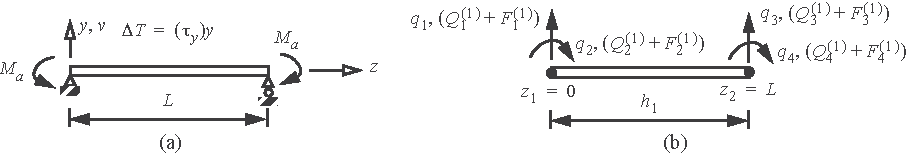
\includegraphics{Figure_17-17.pdf}
}{\caption{(a) Pure bending of a simply supported beam. (b) Finite element model.\label{fig17.17}}}}


The generalized displacement vector $\left\{q^{(1)}\right\}=\left[\begin{array}{@{}llll@{}}q_{1} & q_{2} & q_{3} & q_{4}\end{array}\right]^{T}$ is partitioned to unknown components $\left\{q_{\alpha}\right\}$ and known components $\left\{q_{\beta}\right\}$:
\begin{equation}
\big\{q^{(1)}\big\}=\left[\begin{array}{@{}l@{}}\left\{q_{\alpha}\right\} \\\left\{q_{\beta}\right\}\end{array}\right], \left\{q_{\alpha}\right\}=\left[\begin{array}{@{}l@{}}q_{2} \\q_{4}\end{array}\right], \textrm{ and } \left\{q_{\beta}\right\}=\left[\begin{array}{@{}l@{}}q_{1} \\q_{3}\end{array}\right]=\left[\begin{array}{@{}l@{}}0 \\0\end{array}\right]. \label{eq17.3.a}\tag{a}
\end{equation}
The generalized displacement vector (\ref{eq17.69}) is
\begin{equation}
\left[\begin{array}{@{}l@{}}\phi_{x}^{(1)}(\zeta) \\v(1)(\zeta)\end{array}\right]=\left[\begin{array}{@{}cccc@{}}0 & \eta_{1} & 0 & \eta_{2} \\\eta_{1} & 0 & \eta_{2} & 0\end{array}\right]\left[\begin{array}{@{}c@{}}0 \\q_{2} \\0 \\q_{4}\end{array}\right]+\left[\begin{array}{@{}ccc@{}}0 & \eta_{3} & 0 \\\eta_{3} & 0 & \eta_{4}\end{array}\right]\left[\begin{array}{@{}c@{}}a_{1} \\a_{2} \\a_{3}\end{array}\right]=\left[\begin{array}{@{}c@{}}\eta_{1}(\zeta) q_{2}+\eta_{2}(\zeta) q_{4}+\eta_{3}(\zeta) a_{2} \\\eta_{3}(\zeta) a_{1}+\eta_{4}(\zeta) a_{3}\end{array}\right]. \label{eq17.3.b}\tag{b}
\end{equation}
Displacement boundary conditions $v(-1)=0$ and $v(1)=0$ are satisfied by (\textbf{b}). Matrix (\ref{eq17.106}) represents the unrestrained structural stiffness matrix $\left[K_{u}\right]$. The rows and columns of $\left[K_{u}\right]$ are interchanged to the order 2, 4, 1, and 3 to facilitate partitioning it into submatrices:
\begin{equation}
\left[K_{u}\right]=\mu\left[\begin{array}{@{}cccc@{}}q_{2} & q_{4} & q_{1} & q_{3} \\\frac{12 E I_{x x}}{L}+4 L s_{y y} & \frac{-12 E I_{x x}}{L}+2 L s_{y y} & -6 s_{y y} & 6 s_{y y} \\[6pt]
\frac{-12 E I_{x x}}{L}+2 Ls_{y y} & \frac{12 E I_{x x}}{L}+4 L s_{y y} & -6 s_{y y} & 6 s_{y y} \\[4pt]
\hdashline\\[-8pt]
-6 s_{y y} & -6 s_{y y} & \frac{12 s_{y y}}{L} & \frac{-12 s_{y y}}{L} \\[6pt]
6 s_{y y} & 6 s_{y y} & \frac{-12 s_{y y}}{L} & \frac{12 s_{y y}}{L}\end{array}\right]=\left[\begin{array}{@{}l@{}}{\big[K_{\alpha \alpha}\big]\left[K_{\alpha \beta}\right]} \\{\left[K_{\beta \alpha}\right]\left[K_{\beta \beta}\right]}\end{array}\right]. \label{eq17.3.c}\tag{c}
\end{equation}
The restrained structural stiffness matrix is
\begin{equation}
\left[K_{\alpha \alpha}\right]=\frac{E I_{x x}}{12 E I_{x x}+L^{2} s_{y y}}\left[\begin{array}{@{}ll@{}}\frac{12 E I_{x x}}{L}+4 L s_{y y} & \frac{-12 E I_{x x}}{L}+2 L s_{y y} \\[6pt]
\frac{-12 E I_{x x}}{L}+2 L s_{y y} & \frac{12 E I_{x x}}{L}+4 L s_{y y}\end{array}\right], \label{eq17.3.d}\tag{d}
\end{equation}
where $\mu$ is defined in eq.~(\ref{eq17.103}). From (\ref{eq17.97}) actions $\left.F I_{1}^{(1)}=F I_{2}^{(1)}=F I_{2}^{(1)}\right)=0$, since $f_{y}=0$ and $\tau_{y}$ is spatially uniform in $\zeta$. Hence, from (\ref{eq17.105}) the generalized nodal force vector is $\left\{F^{(1)}\right\}=\left\{F E^{(1)}\right\}$, which is evaluated from (\ref{eq17.97}). The generalized nodal force vector $\left\{Q^{(1)}\right\}=\left[Q_{1}^{(1)} Q_{2}^{(1)} Q_{3}^{(1)} Q_{4}^{(1)}\right]^{T}$ is partitioned into known components $\left\{Q_{0,}\right\}$ and unknown components $\left\{Q_{\beta}\right\}$:
\begin{equation}
\left\{Q_{\alpha}\right\}=\left[\begin{array}{@{}l@{}} Q_{2} \\Q_{4}\end{array}\right]=\left[\begin{array}{@{}c@{}}-M_{a} \\M_{a}\end{array}\right], \textrm{ and } \left\{Q_{\beta}\right\}=\left[\begin{array}{@{}l@{}}Q_{1} \\Q_{3}\end{array}\right]. \label{eq17.3.e}\tag{e}
\end{equation}
The generalized force vector $\left\{F^{(1)}\right\}=\left[\begin{array}{@{}llll@{}}F_{1}^{(1)} & F_{2}^{(1)} & F_{3}^{(1)} & F_{4}^{(1)}\end{array}\right]^{T}$ (\ref{eq17.97}) is prescribed and is partitioned as
\begin{equation}
\left\{F_{\alpha}\right\}=\left[\begin{array}{@{}c@{}}F_{2}^{(1)}\\[4pt]
F_{4}^{(1)}\end{array}\right]=\left[\begin{array}{@{}l@{}}
\int\limits^{1}_{-1}\frac{\left(-E I_{x x} \alpha \tau_{y}\right)}{2} d\zeta \\
\int\limits^{1}_{-1}\frac{\left(E I_{x x} \alpha \tau_{y}\right)}{2} d\zeta \end{array}\right]=\left[\begin{array}{@{}c@{}}-E I_{x x} \alpha \tau_{y} \\E I_{x x} \alpha \tau_{y}\end{array}\right], \textrm{ and } \left\{F_{\beta}\right\}=\left[\begin{array}{@{}l@{}}F_{1}^{(1)} \\[4pt]F_{3}^{(1)}\end{array}\right]=\left[\begin{array}{@{}l@{}}0 \\0\end{array}\right]. \label{eq17.3.f}\tag{f}
\end{equation}
The matrix equation to determine the unknown displacements is $\left[K_{\alpha \alpha}\right]\left\{q_{\alpha}\right\}=\left\{Q_{\alpha}\right\}+\left\{F_{\alpha}\right\}$, or
\begin{equation}
\frac{E I_{x x}}{12 E I_{x x}+L^{2} s_{y y}}\left[\begin{array}{@{}ll@{}}
\frac{12 E I_{x x}}{L}+4 L s_{y y} & \frac{-12 E I_{x x}}{L}+2 L s_{y y} \\[4pt]
\frac{-12 E I_{x x}}{L}+2 L s_{y y} & \frac{12 E I_{x x}}{L}+4 L s_{y y}
\end{array}\right]\left[\begin{array}{@{}l@{}}q_{2} \\[4pt]
q_{4}\end{array}\right]=\left[\begin{array}{@{}c@{}}-M_{a}-E I_{x x} \alpha \tau_{y} \\[4pt]
M_{a}+E I_{x x} \alpha \tau_{y}\end{array}\right]. \label{eq17.3.g}\tag{g}
\end{equation}
The solution for $\left\{q_{\alpha}\right\}$ from eq. (\textbf{\ref{eq17.3.g}}) is
\begin{equation}
\left\{q_{\alpha}\right\}=\left[\begin{array}{@{}l@{}}q_{2} \\q_{4}\end{array}\right]=\frac{L\left(M_{a}+E I_{x x} \alpha \tau_{y}\right)}{2 E I_{x x}}\left[\begin{array}{@{}c@{}}-1 \\1\end{array}\right]. \label{eq17.3.h}\tag{h}
\end{equation}
The rotations are equal magnitude and of the opposite sense. The reactive force vector is determined from $\left[K_{\beta \alpha}\right]\left\{q_{\alpha}\right\}+\left[K_{\beta \beta}\right]\left\{q_{\beta}\right\}=\left\{Q_{\beta}\right\}+\left\{F_{\beta}\right\}$, which is
\begin{equation}
\frac{E I_{x x}}{12 E I_{x x}+L^{2} s_{y y}}\left[\begin{array}{@{}cc@{}}-6 s_{y y} & -6 s_{y y} \\6 s_{y y} & 6 s_{y y}\end{array}\right] \frac{L\left(M_{a}+E I_{x x} \alpha \tau_{y}\right)}{2 E I_{x x}}\left[\begin{array}{@{}c@{}}-1 \\1\end{array}\right]=\frac{L\left(M_{a}+E I_{x x} \alpha \tau_{y}\right)}{2\left(12 E I_{x x}+L^{2} s_{y y}\right)}\left[\begin{array}{@{}c@{}}6 s_{y y}-6 s_{y y} \\-6 s_{y y}+6 s_{y y}\end{array}\right]=\left[\begin{array}{@{}l@{}}0 \\0\end{array}\right]. \label{eq17.3.i}\tag{i}
\end{equation}
Hence, the reactive force vector $\left\{Q_{\beta}\right\}$ vanishes. The vector $\left\{a^{(1)}\right\}$ associated with internal shape function is determined from (\ref{eq17.101}) and (\ref{eq17.102}). These computations are
\begin{equation}
\left\{a^{(1)}\right\}=\left[K_{a a}\right]^{-1}\left\{F I^{(1)}\right\}+\left[G_{a q}\right]\left\{q_{k}\right\}=0_{3 x 1}+\left[\begin{array}{@{}cccc@{}}
0 & \frac{L}{2 \sqrt{6}} & 0 & \frac{-L}{2 \sqrt{6}} \\[7pt]
\frac{-\sqrt{6} L s_{y y}\mu}{E I_{x x}} & \frac{\sqrt{\frac{3}{2}} L^{2} \mu}{E I_{x x}} & \frac{\sqrt{6} L s_{y y} \mu}{E I_{x x}} & \frac{\sqrt{\frac{3}{2}} L^{2} \mu}{E I_{x x}} \\[7pt]
\frac{L^{2} s_{y y} \mu}{\sqrt{10} E I_{x x}} & \frac{-L^{3} s_{y y} \mu}{2 \sqrt{10} E I_{x x}} & \frac{-L^{2} s_{y y} \mu}{\sqrt{10} E I_{x x}} & \frac{-L^{3} s_{y y} \mu}{2 \sqrt{10}EI_{xx}} \end{array}\right]\left[\begin{array}{@{}c@{}}0 \\
q_{2} \\
0 \\
q_{4}\end{array}\right]. \label{eq17.3.j}\tag{j}
\end{equation}
Since $q_{2}=-q_{4}$, we get
\begin{equation}
\left\{a^{(1)}\right\}=\left[\begin{array}{@{}c@{}}\frac{-L}{\sqrt{6}} \\0 \\0\end{array}\right] q_{4}=\left[\begin{array}{@{}c@{}}\frac{-L^{2}\left(M_{a}+E I_{x x} \alpha \tau_{y}\right)}{2 \sqrt{6} E I_{x x}} \\[4pt]0 \\0\end{array}\right]. \label{eq17.3.k}\tag{k}
\end{equation}
The generalized displacement vector in eq. (\textbf{\ref{eq17.3.b}}) is
\begin{equation}
\left[\begin{array}{@{}l@{}}\phi_{x}^{(1)} \\v^{(1)}\end{array}\right]=\left[\begin{array}{@{}c@{}}\frac{L\left(M_{a}+E I_{x x} \alpha \tau_{y}\right) \zeta}{2 E I_{x x}} \\[4pt]\frac{L^{2}\left(M_{a}+E I_{x x} \alpha \tau_{y}\right)\left(1-\zeta^{2}\right)}{8 E I_{x x}}\end{array}\right]. \label{eq17.3.l}\tag{l}
\end{equation}
From (\ref{eq17.110}) the bending moment and shear force are
\begin{equation}
\left[\begin{array}{@{}c@{}}M_{x} \\V_{y}\end{array}\right]=\left[S_{q}\right]\left[\begin{array}{@{}c@{}}0 \\q_{2} \\0 \\q_{4}\end{array}\right]+\left[S_{F}\right]\left[\begin{array}{@{}l@{}}0 \\0 \\0\end{array}\right]-\left[\begin{array}{@{}c@{}}E I_{x x} \alpha \tau_{y} \\0\end{array}\right]=\left[\begin{array}{@{}c@{}}S_{q}\end{array}\right]\left[\begin{array}{@{}c@{}}0 \\-1 \\0 \\1\end{array}\right] q_{4}-\left[\begin{array}{@{}c@{}}E I_{x x} \alpha \tau_{y} \\0\end{array}\right]. \label{eq17.3.m}\tag{m}
\end{equation}
The matrix multiplication of $\left[S_{q}\right]$ times the 4X1 vector in eq. (\textbf{\ref{eq17.3.m}}) is
\begin{align}
&\left[\begin{array}{@{}c@{}cc@{}c@{}}
-6 s_{y y}\mu\zeta & \left(\frac{-E I_{x x}}{L}+3 L s_{y y} \mu \zeta\right) & 6 s_{y y}\mu\zeta &\left(\frac{E I_{x x}}{L}+3 L s_{y y} \mu \zeta\right) \\
\frac{-12\mu s_{y y}}{L} & 6 s_{y y}\mu & \frac{12\mu s_{y y}}{L} & 6 s_{y y}\mu
\end{array}\right] \left[\begin{array}{@{}c@{}}0 \\-1 \\0 \\1\end{array}\right]  \nonumber\\
&\quad=\left[\begin{array}{@{}c@{}}
-\left(-\frac{EI_{x x}}{L}+3\mu\zeta L s_{yy}\right)+\left(\frac{E I_{x x}}{L}+3 \mu \zeta L s_{y y}\right) \\
0
\end{array}\right]. \label{eq17.3.n}\tag{n}
\end{align}
The final result for the bending moment and shear force is\vspace*{4pt}
\begin{equation}
\left[\begin{array}{@{}c@{}} M_{x} \\ V_{y} \end{array}\right]=\left[\begin{array}{@{}c@{}}
\frac{2 E I_{x x}}{L} \\ 0 \end{array}\right] \frac{L\left(M_{a}+E I_{x x} \alpha \tau_{y}\right)}{2 E I_{x x}}-\left[\begin{array}{@{}c@{}} E I_{x x} \alpha \tau_{y} \\ 0 \end{array}\right]=\left[\begin{array}{@{}c@{}} M_{a} \\0 \end{array}\right]. \label{eq17.3.o}\tag{o}
\end{equation}

\vspace*{-8pt}

\noindent The\enlargethispage{1.56\baselineskip} bending moment is constant in the element and it is equal to the prescribed external moment $M_{a}$. The shear force vanishes within the element. If $M_{a}=0$ and $\tau_{y} \neq 0$, then bending moment $M_{x}=0$. However, the rotation and displacement are not zero; i.e.,
\begin{equation}
\left[\begin{array}{@{}l@{}}\phi_{x} \\v\end{array}\right]=\left.\left[\begin{array}{@{}c@{}}\left(L \alpha \tau_{y}\right) \zeta/2 \\\frac{L^{2}}{8} \alpha \tau_{y}\left(1-\zeta^{2}\right)\end{array}\right]\right|_{M_{a}=0}. \label{eq17.3.p}\tag{p}
\end{equation}

\vspace*{-4pt}

\noindent This one-element solution is the same as the exact solution.
\end{example}

\vspace*{-2\baselineskip}

\begin{example}[Transverse bending] \label{ex17.4}
A cantilever, uniform beam of length \textit{L} is subject to a vertical force $F_{a}$ at its free end as shown
 in figure~\ref{fig17.18}. The distributed load intensity $f_{y}=0$, and the through-the-thickness temperature gradient $\tau_{y}(z)=0$, $0<z<L$. One element  models the entire beam as shown in figure~\ref{fig17.17}(b). Since $f_{y}=0$ and $\tau_{y}(z)=0$, prescribed actions (\ref{eq17.97})\begin{wrapfigure}[7]{l}{137pt}
\vspace{-6pt}
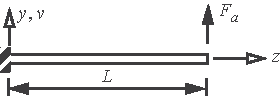
\includegraphics{Figure_17-18.pdf}
\caption{Transverse bending of a cantilever beam.\label{fig17.18}}
%\vspace{-15pt}
\end{wrapfigure} $\left\{F E^{(1)}\right\}=0_{4 X 1}$ and $\left\{F I^{(1)}\right\}=0_{3 X 1}$. It follows from (\ref{eq17.105}) that $\left\{F^{(1)}\right\}=0_{4 X 1}$. The 4X1 generalized nodal displacement vector $\left\{q^{(1)}\right\}$ and the 4X1 generalized force vector $\left\{Q^{(1)}\right\}$ are partitioned into known and unknown components as follows:\vspace*{-8pt}
\begin{align}
\left\{q_{\alpha}\right\} &=\left[\begin{array}{@{}ll@{}}q_{3} & q_{4}\end{array}\right]^{T}, \left\{Q_{\alpha}\right\}=\left[\begin{array}{@{}ll@{}}Q_{3} & Q_{4}\end{array}\right]^{T}=\left[\begin{array}{@{}ll@{}}F_{a} & 0\end{array}\right]^{T},\nonumber\\
\left\{q_{\beta}\right\} &=\left[\begin{array}{@{}ll@{}}q_{1} & q_{2}\end{array}\right]^{T}=0_{2 X 1}, \textrm{ and } \left\{Q_{\beta}\right\}=\left[\begin{array}{@{}ll@{}}Q_{1} & Q_{2}\end{array}\right]^{T}. \label{eq17.4.a}\tag{a}
\end{align}

\pagebreak
\noindent Matrix (\ref{eq17.106}) represents the unrestrained structural stiffness matrix $\left[K_{u}\right]$. The rows and columns of $\left[K_{u}\right]$ are interchanged to the order 3, 4, 1, and 2 to facilitate partitioning it into submatrices:
\begin{equation}
\left[K_{u}\right]=\mu
\begin{array}{@{}c@{}}
\begin{array}{@{}cccc@{}}
q_{3} & q_{4} & q_{1} & q_{2} \\[5pt]
\phantom{6 s_{y y}} & \phantom{\frac{12 E I_{x x}}{L}+4 L s_{y y}} & \phantom{-6 s_{y y}} & \phantom{\frac{-12 E I_{x x}}{L}+2 L s_{y y}} \\
\end{array}
\\[-12pt]
\left[\begin{array}{@{\ }cc;{2pt/2pt}cc@{\ }}
\frac{12 s_{y y}}{L} & 6 s_{y y} & \frac{12 s_{y y}}{L} & 6 s_{y y} \\
6 s_{y y} & \frac{12 E I_{x x}}{L}+4 L s_{y y} & -6 s_{y y} & \frac{-12 E I_{x x}}{L}+2 L s_{y y} \\[3pt]\hdashline & & & \\[-8pt]
\frac{12^{\vphantom{M}} s_{y y}}{L} & -6 s_{y y} & \frac{12 s_{y y}}{L} & -6 s_{y y} \\6 s_{y y} & \frac{-12 E I_{x x}}{L}+2 L s_{y y} & -6 s_{y y} & \frac{12 E I_{x x}}{L}+4 L s_{y y}\end{array}\right]
\end{array}
=\left[\begin{array}{@{}l@{}}{\left[K_{\alpha \alpha}\right]\left[K_{\alpha \beta}\right]} \\{\left[K_{\beta \alpha}\right]\left[K_{\beta \beta}\right]}\end{array}\right]. \label{eq17.4.b}\tag{b}
\end{equation}
The matrix equation to determine the unknown displacements is $\left[K_{\alpha \alpha}\right]\left\{q_{\alpha}\right\}+\left[K_{\alpha\beta}\right]\left\{q_{\beta}\right\}=\left\{Q_{\alpha}\right\}$, or
\begin{equation}
\frac{E I_{x x}}{12 E I_{x x}+L^{2} s_{y y}}\left[\begin{array}{@{}cc@{}}\frac{12 s_{y y}}{L} & 6 s_{y y} \\[4pt]
6 s_{y y} & \frac{12 E I_{x x}}{L}+4 L s_{y y}\end{array}\right]\left[\begin{array}{@{}l@{}}q_{3} \\q_{4}\end{array}\right]=\left[\begin{array}{@{}c@{}}F_{a} \\0\end{array}\right]. \label{eq17.4.c}\tag{c}
\end{equation}
The solution of eq. (\textbf{\ref{eq17.4.c}}) for the displacements is
\begin{equation}
\left[\begin{array}{@{}l@{}}q_{3} \\q_{4}\end{array}\right]=\left[\begin{array}{@{}c@{}}\frac{F_{a} L^{3}}{3 E I_{x x}}+\frac{F_{a} L}{s_{y y}} \\[4pt]
\frac{-F_{a} L^{2}}{2 E I_{x x}}\end{array}\right]. \label{eq17.4.d}\tag{d}
\end{equation}
The matrix formulation to determine the generalized reactive force vector is $\left[K_{\beta \alpha}\right]\left\{q_{\alpha}\right\}+\left[K_{\beta \beta}\right]\left\{q_{\beta}\right\}=\left\{Q_{\beta}\right\}$, or
\begin{equation}
\left[\begin{array}{@{}l@{}}Q_{1} \\Q_{2}\end{array}\right]=\mu\left[\begin{array}{@{}cc@{}}\frac{-12 s_{y y}}{L} & -6 s_{y y} \\6 s_{y y} & \frac{-12 E I_{x x}}{L}+2 L s_{y y}\end{array}\right]\left[\begin{array}{@{}c@{}}\frac{L^{2}}{3 E I_{x x}}+\frac{1}{s_{y y}} \\[4pt]
\frac{-L}{2 E I_{x x}}\end{array}\right] F_{a} L=\mu L F_{a}\left[\begin{array}{@{}c@{}}\frac{-\left(12 E I_{x x}+L^{2} s_{y y}\right)}{E I_{x x} L} \\[4pt]
\frac{12 E I_{x x}+L^{2} s_{y y}}{E I_{x x}}\end{array}\right]=\left[\begin{array}{@{}l@{}}-F_{a} \\L F_{a}\end{array}\right]. \label{eq17.4.e}\tag{e}
\end{equation}
The generalized displacement vector $\left\{a^{(1)}\right\}$ associated with internal shape function is determined from (\ref{eq17.101}) and (\ref{eq17.102}). The result is
\begin{equation}
\left\{a^{(1)}\right\}=\left[K_{a a}\right]^{-1}\left\{F I^{(1)}\right\}+\left[G_{a q}\right]\left\{q_{k}\right\}=0_{3 X 1}+\left[G_{a q}\right]
\left[\begin{array}{@{}l@{}}0 \\0 \\q_{3} \\q_{4}\end{array}\right]=
\left[\begin{array}{@{}c@{}}\frac{F_{a} L^{3}}{4 \sqrt{6} E I_{x x}} \\[6pt]\frac{F_{a} L^{2}}{2 \sqrt{6} E I_{x x}} \\[6pt]\frac{-F_{a} L^{3}}{12 \sqrt{10} E I_{x x}}\end{array}\right]. \label{eq17.4.f}\tag{f}
\end{equation}
The generalized displacement vector (\ref{eq17.70}) is
\begin{equation}
\left[\begin{array}{@{}l@{}}\phi_{x}^{(1)} \\[4pt]v^{(1)}\end{array}\right]=\left[\begin{array}{@{}cccc@{}}0 & \eta_{1} & 0 & \eta_{2} \\\eta_{1} & 0 & \eta_{2} & 0\end{array}\right]\left[\begin{array}{@{}c@{}}0 \\0 \\q_{3} \\ q_{4} \end{array}\right]+\left[\begin{array}{@{}ccc@{}} 0 & \eta_{3} & 0 \\ \eta_{3} & 0 & \eta_{4} \end{array}\right]\left[\begin{array}{@{}l@{}} a_{1}^{(1)} \\[4pt] a_{2}^{(1)} \\[4pt] a_{3}^{(1)} \end{array}\right]=\left[\begin{array}{@{}c@{}} \frac{F_{a} L^{2}}{8 E I_{x x}}\left(-3-2 \zeta+\zeta^{2}\right) \\[6pt] \frac{F_{a} L(1+\zeta)\left[24 E I_{x x}+L^{2} s_{y y}\left(5+4 \zeta-\zeta^{2}\right)\right]}{48 E I_{x x} s_{y y}} \end{array}\right]. \label{eq17.4.g}\tag{g}
\end{equation}
The vector of the bending moment and shear force (\ref{eq17.110}) is
\begin{equation}
\left[\begin{array}{@{}c@{}}M_{x} \\V_{y}\end{array}\right]=\left[S_{q}\right]\left[\begin{array}{@{}c@{}}0 \\0 \\q_{3} \\q_{4}\end{array}\right]=\left[\begin{array}{@{}c@{}}\left(6 \mu s_{y y} \zeta\right)\left(\frac{F_{a} L^{3}}{3 E I_{x x}}+\frac{F_{a} L}{s_{y y}}\right)+\left(\frac{E I_{x x}}{L}+3 \mu L_{k} s_{y y} \zeta\right)\left(\frac{-F_{a} L^{2}}{2 E I_{x x}}\right) \\[6pt]
\left(12 \mu s_{y y}\right)\left(\frac{F_{a} L^{3}}{3 E I_{x x}}+\frac{F_{a} L}{s_{y y}}\right)+\left(6 \mu s_{y y}\right)\left(\frac{-F_{a} L^{2}}{2 E I_{x x}}\right)\end{array}\right]=\left[\begin{array}{@{}c@{}}\frac{F_{a} L(-1+\zeta)}{2} \\[4pt]F_{a}\end{array}\right]. \label{eq17.4.h}\tag{h}
\end{equation}
The shear force is constant in the beam and is equal to the prescribed external force $F_{\textrm{a}}$. For $F_{a}>0$ the bending moment decreases linearly from zero at the free end to a minimum ($-F_{a} L$) at the clamped end. The finite element solution for transverse bending is the same as the exact solution of the governing boundary value problem.
\end{example}


\vspace*{-1pc}



\begin{example}[Cantilever wing spar]\label{ex17.5}The wing spar of a light airplane described in example~\ref{ex6.6} on page~\pageref{ex6.6} is modeled as a cantilever beam as shown in figure~\ref{fig17.19}(a). In a symmetric maneuver of the airplane the total lift $L=12{,}000$~lb., and the lift acting on each wing is \textit{L/2}. Assume the airload acts along the locus of shear centers so that spar bends without twist in torsion. The airload is distributed elliptically over the wing, so that the airload intensity $f_{y}(z)$ per unit span is given as
{\def\thefigure{17.19}
\processfigure{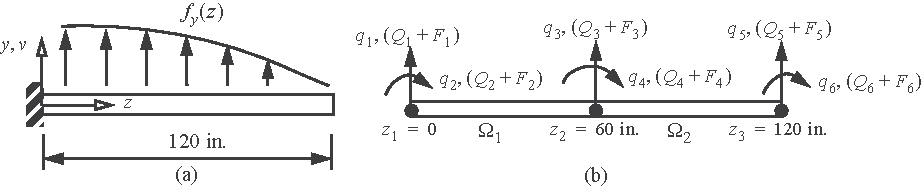
\includegraphics{Figure_17-19.pdf}
}{\caption{(a) Cantilever wing spar. (b) Finite element model.\label{fig17.19}}}}
\begin{equation}
f_{y}(z)=\frac{2 L}{\pi z_{m a x}} \sqrt{1-\left(\frac{z}{z_{m a x}}\right)^{2}} \quad 0 \leq z \leq z_{\max}, \label{eq17.5.a}\tag{a}
\end{equation}
where $z$ is the spanwise coordinate, $z=0$ at the root, and $z=z_{\max}=120\,\mathrm{in}$ at the tip of the wing spar. The transverse temperature gradient $\tau_{y}(z)=0$, $0<z<z_{\max}$. Data taken from example~\ref{ex6.6} are: the modulus of elasticity $E=10.5 \times 10^{6}\,\mathrm{lb}./\text { in. }^{2}$, the second area moment of the cross section about the $x$-axis $I_{x x}=101.619\,\mathrm{in}^{4}$, and the transverse shear coefficient $s_{y y}=2.4278 \times 10^{6}\,\mathrm{lb}$

The finite element model shown in figure~\ref{fig17.19}(b) has three nodes $\left\{z_{3}\right\}=\{0,60,120\} \text { in. }$, and two equal length elements $h_{1}=h_{2}=60\,\mathrm{in}$. The stiffness matrices (\ref{eq17.106}) for each element are
\begin{gather}
\left[K^{(1)}\right]=\left[\begin{array}{@{}cccc@{}}q_{1} & q_{2} & q_{3} & q_{4} \\24,048 & -721,441 & -24,048 & -721,441 \\-721,441 & 3.94266 \times 10^{7} & 721,441 & 3.85991 \times 10^{6} \\-24,048 & 721,441 & 24,048 & 721,441 \\-721,441 & 3.85991 \times 10^{6} & 721,441 & 3.94266 \times 10^{7}\end{array}\right] \textrm{ and}\label{eq17.5.b}\tag{b}\\
\left[K^{(2)}\right]=\left[\begin{array}{@{}cccc@{}}q_{3} & q_{4} & q_{4} & q_{5} \\24,048 & -721,441 & -24,048 & -721,441 \\-721,441 & 3.94266 \times 10^{7} & 721,441 & 3.85991 \times 10^{6} \\-24,048 & 721,441 & 24,048 & 721,441 \\-721,441 & 3.85991 \times 10^{6} & 721,441 & 3.94266 \times 10^{7}\end{array}\right].  \label{eq17.5.c}\tag{c}
\end{gather}
The assembly process effects the matrix addition $\left[K_{u}\right]=\left[K^{(1)}\right]+\left[K^{(2)}\right]$ to get the unrestrained structural stiffness matrix as\pagebreak
\begin{equation}
\left[K_{u u}\right]=\left[\begin{array}{@{}cccccc@{}}q_{1} & q_{2} & q_{3} & q_{4} & q_{5} & q_{6} \\24,048 & -721,441 & -24,048 & -721441 . & 0 & 0 \\-721,441 & 3.94266 \times 10^{7} & 721441 & 3.85991 \times 10^{6} & 0 & 0 \\[3pt]
\hdashline\\[-8pt]
-24,048 & 721,441 & 48,096.1 & 0 & -24,048 & -721441 . \\[3pt]\hdashline\\[-8pt] 721,441 & 3.85991 \times 10^{6} & 0 & 7.88531 \times 10^{7} & 721,441 & 3.85991 \times 10^{6} \\0 & 0 & -24,048 & 721,441 & 24,048 & 721,441 \\0 & 0 & -721,441 & 3.85991 \times 10^{6} & 721,441 & 3.94266 \times 10^{7}\end{array}\right]. \label{eq17.5.d}\tag{d}
\end{equation}
The generalized nodal displacement vector $\left[\begin{array}{@{}llllll@{}}q_{1} & q_{2} & q_{3} & q_{4} & q_{5} & q_{6}\end{array}\right]^{T}$ is partitioned into unknown components $\left\{q_{\alpha}\right\}$ and known components $\left\{q_{\beta}\right\}$:
\begin{equation}
\left\{q_{\alpha}\right\}=\left[\begin{array}{@{}llll@{}}q_{3} & q_{4} & q_{5} & q_{6}\end{array}\right]^{T} \quad\left\{q_{\beta}\right\}=\left[\begin{array}{@{}ll@{}}q_{1} & q_{2}\end{array}\right]^{T}=0_{2 X 1}. \label{eq17.5.e}\tag{e}
\end{equation}
We partition the unrestrained structural stiffness in eq. (\textbf{\ref{eq17.5.d}}) in the form
\begin{align}
\left[K_{u}\right]=\left[\begin{array}{@{}ll@{}}{\left[K_{\beta \beta}\right]} & {\left[K_{\beta \alpha}\right]} \\[4pt]{\left[K_{\alpha \beta}\right]} & {\left[K_{\alpha \alpha}\right]}\end{array}\right], \textrm{ where}\label{eq17.5.f}\tag{f}
\end{align}
\begin{align}
\left[K_{\alpha \alpha}\right]&=
\left[\begin{array}{@{}cccc@{}}
q_{3} & q_{4} & q_{5} & q_{6} \\[4pt]48,096.1 & 0 & -24,048 & -721,441 \\[4pt]0 & 7.88531 \times 10^{7} & 721,441 & 3.85991 \times 10^{6} \\[4pt]-24,048 & 721,441 & 24,048 & 721,441 \\[4pt]-721,441 & 3.85991 \times 10^{5} & 721,441 & 3.94266 \times 10^{7}\end{array}\right],\nonumber\\
\left[K_{\alpha \beta}\right]
&=
\begin{array}{@{}c@{}}
\begin{array}{@{}c@{\qquad}c@{}}
q_{1} & q_{2}
\end{array}\\[4pt]
\left[\begin{array}{@{}cc@{}}
-24,048 & 721,441 \\[4pt]
-721,441 & 3.85991 \times 10^{6} \\[4pt]
0 & 0 \\[4pt]
0 & 0
\end{array}\right]\\
\end{array}
=\left[K_{\beta \alpha}\right]^{T}\!, \label{eq17.5.g}\tag{g}
\end{align}
and
{\def\thefigure{17.20}
\processfigure[b]{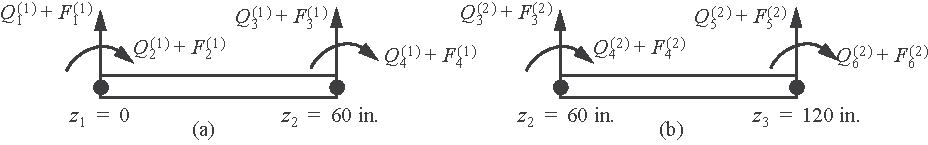
\includegraphics{Figure_17-20.pdf}
}{\caption{Generalized forces acting on (a) element $\Omega_1$, and (b) element $\Omega_2$.\label{fig17.20}}}}
\begin{equation}
\left[K_{\beta \beta}\right]=\left[\begin{array}{@{}cc@{}}q_{1} & q_{2} \\
24,048 & -721,441 \\-721,441 & 3.94266 \times 10^{7}\end{array}\right]. \label{eq17.5.h}\tag{h}
\end{equation}
The generalized forces acting at the nodes of elements 1 and 2 are shown in figure~\ref{fig17.20}. The external generalized forces acting on elements $\Omega_1$ and $\Omega_2$ from the distributed airload (\textbf{\ref{eq17.5.a}}) are computed by numerical integration because of the complexity of the integrands (\ref{eq17.97}). (Refer to article~\ref{sec17.3.6} for details on numerical integration.) The external generalized forces acting on each element are determined from eq.~(\ref{eq17.105}). The transpose of the Guyan matrix used to compute the generalized force vectors $\left\{F^{(1)}\right\}$ and $\left\{F^{(2)}\right\}$ in eq.~(\ref{eq17.105}) is the same for each element in this example. It is given by
\begin{equation}
\left[G_{a q}^{(1)}\right]^{T}=\left[G_{a q}^{(2)}\right]^{T}=\left[\begin{array}{@{}ccc@{}} 0 & -0.016526 & 0.128289 \\12.2474 & 0.496859 & -3.84866 \\ 0 & 0.016562 & -0.128289 \\ -12.2474 & 0.496859 & -3.84866\end{array}\right]. \label{eq17.5.i}\tag{i}
\end{equation}
The results for the generalized forces are
\begin{gather}
\left\{F E^{(1)}\right\} \equiv\left[\begin{array}{@{}c@{}}1,869\,\mathrm{lb}. \\0 \\1,784.98\,\mathrm{lb}. \\0\end{array}\right] \quad\left\{F I^{(1)}\right\} \equiv\left[\begin{array}{@{}c@{}}-1,499.03\,\mathrm{lb}. \\0 \\266.3992\,\mathrm{lb}.\end{array}\right] \quad\left\{F^{(1)}\right\}=\left[\begin{array}{@{}c@{}}F_{1}^{(1)} \\F_{2}^{(1)} \\F_{3}^{(1)} \\F_{4}^{(1)}\end{array}\right]=\left[\begin{array}{@{}c@{}}1,872.39\,\mathrm{lb}. \\-18,460.9\,\mathrm{lb}.\mathrm{-in}. \\1,781.6\,\mathrm{lb}. \\18,257.7\,\mathrm{lb}.\mathrm{-in}.\end{array}\right], \label{eq17.5.j}\tag{j} \\
\left\{F E^{(2)}\right\} \equiv\left[\begin{array}{@{}c@{}}1,384.05\,\mathrm{lb}. \\0 \\961.96\,\mathrm{lb}. \\0\end{array}\right] \quad\left\{F I^{(2)}\right\} \equiv\left[\begin{array}{@{}c@{}}-991.799\,\mathrm{lb}. \\0 \\125.595\,\mathrm{lb}.\end{array}\right], \textrm{ and } \left\{F^{(2)}\right\}=\left[\begin{array}{@{}c@{}}F_{3}^{(2)} \\F_{4}^{(2)} \\F_{5}^{(2)} \\F_{6}^{(2)}\end{array}\right]=\left[\begin{array}{@{}c@{}}1,400.17\,\mathrm{lb}. \\-12,630.4\,\mathrm{lb}\mathrm{-in}. \\945.848\,\mathrm{lb}. \\11,663.6\,\mathrm{lb}.\mathrm{-in}.\end{array}\right]. \label{eq17.5.k}\tag{k}
\end{gather}
Assembly of the two elements is shown in figure~\ref{fig17.19}(b). The external generalized force vectors for the assembly are
\begin{equation}
\left[\begin{array}{@{}c@{}}F_{1} \\
F_{2} \\
F_{3} \\
F_{4} \\
F_{5} \\
F_{6}\end{array}\right]=\left[\begin{array}{@{}c@{}}F_{1}^{1)} \\
F_{2}^{(1)} \\
F_{3}^{(1)}+F_{3}^{(2)} \\
F_{4}^{(1)}+F_{4}^{(2)} \\
F_{5}^{(2)} \\
F_{6}^{(2)}\end{array}\right]=\left[\begin{array}{@{}c@{}}1,872.39\,\mathrm{lb}. \\
-18,460.9\,\mathrm{lb}.\,\mathrm{in}. \\
3,181.77\,\mathrm{lb}. \\
5,627.30\,\mathrm{lb}.\,\mathrm{in}. \\
945.848\,\mathrm{lb}. \\
11,663.6\,\mathrm{lb}.\,\mathrm{in}.\end{array}\right]\left[\begin{array}{@{}c@{}}Q_{1} \\
Q_{2} \\
Q_{3} \\
Q_{4} \\
Q_{5} \\
Q_{6}\end{array}\right]=\left[\begin{array}{@{}c@{}}Q_{1}^{(1)} \\[4pt]
Q_{2}^{(2)} \\[4pt]
Q_{3}^{(1)}+Q_{3}^{(2)} \\[4pt]
Q_{4}^{(1)}+Q_{4}^{(2)} \\[4pt]
Q_{5}^{(2)} \\[4pt]
Q_{6}^{(2)}\end{array}\right]. \label{eq17.5.l}\tag{l}
\end{equation}
The 6X1 generalized nodal force vector $\left[\begin{array}{@{}llllll@{}}Q_{1} & Q_{2} & Q_{3} & Q_{4} & Q_{5} & Q_{6}\end{array}\right]^{T}$ is partitioned into known components $\left\{Q_{\alpha}\right\}$ and unknown components $\left\{Q_{\beta}\right\}$ as follows:
\begin{equation}
\left\{Q_{\alpha}\right\}=\left[\begin{array}{@{}llll@{}} Q_{3} & Q_{4} & Q_{5} & Q_{6}\end{array}\right]^{T}=0_{4 X 1}, \textrm{ and } \left\{Q_{\beta}\right\}=\left[Q_{1}\ \ Q_{2}\right]^{T}. \label{eq17.5.m}\tag{m}
\end{equation}
There are no generalized point forces acting at nodes 2 and 3. Generalized point forces acting at node 1 are reactive. The generalized forces from the airload are also partitioned as
\begin{gather}
\left\{F_{\alpha}\right\}=\left[\begin{array}{@{}llll@{}}F_{3} & F_{4} & F_{5} & F_{6}\end{array}\right]^{T}=\left[\begin{array}{@{}llll@{}}3,181.76 & 5,627.37 & 945.848 & 11,663.6\end{array}\right]^{T}, \textrm{ and}\label{eq17.5.n}\tag{n}\\
\left\{F_{\beta}\right\}=\left[\begin{array}{@{}ll@{}}F_{1} & F_{2}\end{array}\right]^{T}=[1,872.39-18,460.9]^{T}. \label{eq17.5.o}\tag{o}
\end{gather}

\vspace*{-1pc}

The matrix equation to determine the unknown generalized displacements is $\left[K_{\alpha \alpha}\right]\left\{q_{\alpha}\right\}+\left[K_{\alpha \beta}\right]\left\{q_{\beta}\right\}=\left\{Q_{\alpha}\right\}+\left\{F_{\alpha}\right\}$.The solution for the unknown displacement vector is
\begin{equation}
\left\{q_{\alpha}\right\}=\left[\begin{array}{@{}llll@{}}0.447103 & -0.0091821 & 1.06555 & -0.0101218\end{array}\right]^{T}. \label{eq17.5.p}\tag{p}
\end{equation}
The matrix equation to determine the unknown forces is $\left[K_{\beta \alpha}\right]\left\{q_{\alpha}\right\}+\left[K_{\beta \beta}\right]\left\{q_{\beta}\right\}=\left\{Q_{\beta}\right\}+\left\{F_{\beta}\right\}$, or
\begin{equation}
\left[\begin{array}{@{}cccc@{}}-24,048 & -721,441 & 0 & 0 \\721,441 & 3.85991 \times 10^{6} & 0 & 0\end{array}\right]\left[\begin{array}{@{}c@{}}0.447103 \\-0.0091821 \\1.06555 \\-0.0101218\end{array}\right]+\left[\begin{array}{@{}cc@{}}24,048 & -721,441 \\-721,441 & 3.94266 \times 10^{7}\end{array}\right]\left[\begin{array}{@{}l@{}}0 \\0\end{array}\right]=\left[\begin{array}{@{}l@{}}Q_{1} \\Q_{2}\end{array}\right]+\left[\begin{array}{@{}c@{}}1,872.39 \\-18,460.9\end{array}\right]. \label{eq17.5.q}\tag{q}
\end{equation}
Perform the matrix algebra in eq. (\textbf{\ref{eq17.5.q}}) to find that the generalized reactive forces are
\begin{equation}
Q_{1}=-6{,}000.0\,\mathrm{lb}. \quad Q_{2}=305,577\,\mathrm{lb} \cdot-\mathrm{in}. \label{eq17.5.r}\tag{r}
\end{equation}
The external generalized forces acting on the two-element model of wing spar are shown in the free body diagram in figure~\ref{fig17.21}.
\end{example}
\vspace*{-1\baselineskip}

{\def\thefigure{17.21}
\processfigure{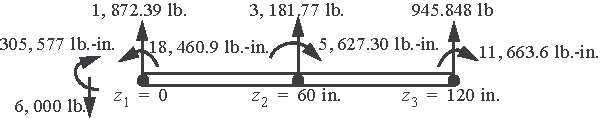
\includegraphics{Figure_17-21.pdf}
}{\caption{Generalized forces acting on the model with two elements.\label{fig17.21}}}}


\subsection{Gaussian integration}\label{sec17.3.6}

Consider the integral to compute the external force component $F E_{2k+1}^{(k)}$ in eq.~(\ref{eq17.97}) for element two in example~\ref{ex17.5}. The expression for this force component is
\begin{align}\label{eq17.116}
F E_{5}^{(2)}=\frac{h_{2}}{2} \int_{-1}^{1} \frac{1}{2}(1+\zeta) \frac{2 L}{\pi z_{max }} \sqrt{1-\left(\frac{z^{(2)}(\zeta)}{z_{max }}\right)^{2}} d \zeta,
\end{align}
where
\begin{align}\label{eq17.117}
z^{(2)}=\eta_{1}(\zeta)(60 .)+\eta_{2}(\zeta)(120)=90+30 \zeta.
\end{align}
Numerical evaluation of eq.~(\ref{eq17.116}) leads to
\begin{align}\label{eq17.118}
F E_{5}^{(2)}=\int_{-1}^{1}\left[954.930(1+\zeta) \sqrt{0.4357-0.375 \zeta-0.0625 \zeta^{2}}\right] d \zeta.
\end{align}
We carry out Gaussian integration of eq.~(\ref{eq17.118}) after a discussion of the method.

The method of Gaussian quadrature is to approximate the integral $I=\int_{-1}^{1} f(\zeta) d \zeta$ by
\begin{align}\label{eq17.119}
I \approx I_{\text {appr }}=\sum_{i=1}^{n s} w_{i} f\left(\zeta_{j i}\right),
\end{align}
where $\zeta_{i}$ are the abscissas of the Legendre polynomial $P_{i}(\zeta)$, and $w_{i}$ are the weight factors. The abscissas, or roots, of the Legendre polynomial are symmetrically located in the interval $-1 \leq \zeta \leq 1$. The weight factors are determined such that a polynomial of degree $p$ is exactly equal to the sum in (\ref{eq17.119}). Consider a polynomial of second degree $f(\zeta)=c_{0}+c_{1} \zeta+c_{2} \zeta^{2}$. The exact integral is
\begin{align}\label{eq17.120}
I=\int_{-1}^{1}\left(c_{0}+c_{1} \zeta+c_{2} \zeta^{2}\right) d \zeta=2 c_{0}+\frac{2}{3} c_{2}.
\end{align}
The exact integral is determined by two coefficients, $c_0$ and $c_2$. The Legendre polynomial for $n=2$ is $P_{2}(\zeta)=\left(-1+3 \zeta^{2}\right)/2$. The roots of $P_{2}(\zeta)=0$ are
\begin{align}\label{eq17.121}
-1/\sqrt{3} \textrm{ and } 1 /(\sqrt{3}).
\end{align}
Equation (\ref{eq17.119}) for $n=2$ is
\begin{align}\label{eq17.122}
I=I_{\text {appr. }}=w_{1} f\left(\frac{-1}{\sqrt{3}}\right)+w_{2} f\left(\frac{1}{\sqrt{3}}\right).
\end{align}
Evaluating eq.~(\ref{eq17.122}) we get
\begin{align}\label{eq17.123}
I=I_{\text {appr. }}=2\left(w_{1}+w_{2}\right) c_{0}+\frac{\left(w_{2}-w_{1}\right)}{\sqrt{3}} c_{1}+\frac{1}{3}\left(w_{1}+w_{2}\right).
\end{align}
Equate like coefficients in (\ref{eq17.120}) and (\ref{eq17.123}) to get three linear equations for the weight factors $w$1, and $w$2:
\begin{align}\label{eq17.124}
2=w_{1}+w_{2} \quad 0=\left(w_{2}-w_{1}\right) /(\sqrt{3}) \quad \frac{2}{3}=\frac{1}{3}\left(w_{1}+w_{2}\right).
\end{align}
The solution of eq.~(\ref{eq17.124}) is $w_{1}=w_{2}=1$. Note that the weight factors of the positive root and the corresponding negative root are the same because the term with the odd power of $\zeta$ does not contribute to \textit{I} (\ref{eq17.120}). Thus, a polynomial of degree 2 can be integrated exactly by evaluating it at $\mp 1/\sqrt{3}$ and multiplying by the appropriate equal weight factors.

Consider the cubic polynomial $f(\zeta)=c_{0}+c_{1} \zeta+c_{2} \zeta^{2}+c_{3} \zeta^{3}$ whose exact integral is $I=2 c_{0}+(2/3) c_{2}$. The Legendre polynomial for $n$ = 3 is $P_{3}(\zeta)=\left(-3 \zeta+5 \zeta^{3}\right)/2$. The roots of $P_{3}(\zeta)=0$ are $0$, and $\mp \sqrt{3/5}$. Equation (\ref{eq17.119}) for $n=3$ is
\begin{align}\label{eq17.125}
I=I_{\text {appr. }}=w_{1} f(0)+w_{2} f(-\sqrt{3/5})+w_{2} f(\sqrt{3/5})=c_{0}\left(w_{1}+w_{2}\right)+c_{2}\left(6 w_{2}/ 5\right).
\end{align}
Equating like coefficients between the last equation and the exact integral we find the weight factors $w_{1}=8/9$ and $w_{2}=5/9$. In general, a polynomial of degree $p$ is integrated exactly if $n \geq(p+1)/2$.

Now consider the integrand in the definite integral (\ref{eq17.118}). The integrand is
\begin{align}\label{eq17.126}
f(\zeta)=954.930(1+\zeta) \sqrt{0.4357-0.375 \zeta-0.0625 \zeta^{2}}.
\end{align}
Function $f(\zeta)$ is continuous in the interval $|\zeta| \leq 1$ as shown in figure~\ref{fig17.22}. Its Taylor's formula is an infinite series $f(\zeta)=\sum_{m=0}^{\infty} a_{m} \zeta^{m}$, where the $a_{m}$ are real numbers. Consequently if $f(\zeta)$ is replaced by its Taylor series, then the integrand is a polynomial of infinite degree. The integral of a polynomial of infinite degree implies an infinite number of abscissas and weights for Gaussian quadrature, which, of course, is not practical. Only a finite number of abscissas and weights in Gaussian quadrature are considered in the sequence of numerical integrations to follow.

Gaussian quadrature of the integrand (\ref{eq17.119}) for $n=2$ is
\begin{align}\label{eq17.127}
I_{\text {appr. }}=w_{1} f(-1/\sqrt{3})+w_{1} f(1/\sqrt{3})=(1)(321.154)+(1)(673.889)=995.043\,\mathrm{lb}
\end{align}
Gaussian quadrature of the integrand (\ref{eq17.119}) for $n=3$ is
\begin{align}\label{eq17.128}
I_{\text {appr. }}=w_{1} f(0)+w_{2} f\left(-\sqrt{\frac{3}{5}}\right)+w_{2} f\left(\sqrt{\frac{3}{5}}\right)=\left(\frac{8}{9}\right)(631.627)+\left(\frac{5}{9}\right)(178.857)+\left(\frac{5}{9}\right)(560.829)=972.382\,\mathrm{lb}
\end{align}
For $n=2$, 3, 4, 5, 6, 7, 8, 9, and 10 the abscissa and weight factors are listed in table~\ref{tab17.4}. Approximate values of the integrals of (\ref{eq17.126}) are listed in table~\ref{tab17.5} based on the data in table~\ref{tab17.4}. The results in table~\ref{tab17.5} show the integrals are slowly decreasing as the number of terms in the Gaussian integration increase. Apparently, the approximate values of the integrals are asymptotically approaching the value of 961.96~lb., which is the value of the integral of (\ref{eq17.126}) computed from the function \textbf{NIntegrate[$f(\zeta), \{\zeta, -1, 1\}$]} in \textit{Mathematica}.

{\def\thefigure{17.22}
\processfigure[t]{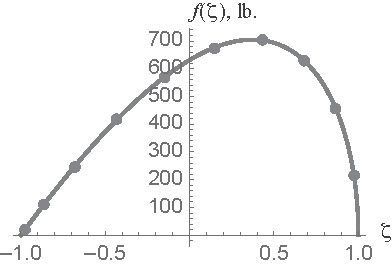
\includegraphics{Figure_17-22.pdf}
}{\caption{Graph of function (17.126) with the filled circles corresponding to the function evaluated at the abscissas in Gaussian quadrature for $\textrm{n} = 10$.\label{fig17.22}}}}

\begin{table}%17.4
\processtable{Abscissas and weight factors for Gaussian integration \label{tab17.4}}{%
\begin{tabular}{@{\extracolsep\fill}llll@{\extracolsep\fill}}
\toprule
\multicolumn{1}{c}{\colhead{$\pm \zeta_{i}$}} & \multicolumn{1}{c}{\colhead{$w_{i}$}} & \multicolumn{1}{c}{\colhead{$\pm\zeta_{i}$}} & \multicolumn{1}{c}{\colhead{$w_{i}$}} \\
\midrule
\multicolumn{2}{c}{$n=2$} & \multicolumn{2}{c}{$n=8$} \\
\midrule
\multicolumn{1}{c}{$1 /(\sqrt{3})$} & \multicolumn{1}{c}{$1.0$} & 0.18343 46424 95650 & 0.36268 37833 78362 \\
\multicolumn{2}{@{}c}{\hrulefill} & 0.52553 24099 16329 & 0.31370 66458 77877 \\
\multicolumn{2}{c}{$n=3$} & 0.79666 64774 13627 & 0.22238 10344 53374  \\
\multicolumn{2}{@{}c}{\hrulefill} & 0.96028 98564 97536  & 0.10122 85362 90376 \\
\multicolumn{1}{c}{0} & \multicolumn{1}{c}{$8/9$} &   &  \\
\multicolumn{1}{c}{$\sqrt{3/5}$} & \multicolumn{1}{c}{$5/9$} &  & \\
\midrule
\multicolumn{2}{c}{$n=4$} & \multicolumn{2}{c}{$n=9$} \\
\midrule
0.33998 10435 84856  &  0.65214 51548 62546  &  0  &  0.33023 93550 01260 \\
0.86113 63115 94053  &  0.34785 48451 37454  &  0.32425 34234 03809  &  0.31234 7 0770 40003\\
\multicolumn{2}{@{}c}{\hrulefill} & 0.61337 14327 0 0590 & 0.26061 06964 02935\\
\multicolumn{2}{c}{$n=5$} & 0.83603 11073 26636 & 0.18064 81606 94857 \\
\multicolumn{2}{@{}c}{\hrulefill} & 0.96816 02395 07626 & 0.08127 43883 61574\\
0 & 0.56888 88888 88889  &    &  \\
0.53846 93101 05683  &  0.47862 86704 99366  &   \multicolumn{2}{@{}c@{}}{\hrulefill} \\
0.90617 98459 38664 & 0.23692 68850 56189 &  \multicolumn{2}{c}{$n=10$}\\
\midrule
\multicolumn{2}{c}{$n=6$} & 0.14887 43389 81631 &  0.29552 42247 14753\\
\multicolumn{2}{@{}c}{\hrulefill} &  0.43339 53941 29247  &  0.26926 67193 09996\\
0.23861 91860 83197 &  0.46791 39345 72691 &  0.67940 95682 99024  & 0.21908 63625 15982\\
0.66120 93864 66265 &  0.36076 15730 4 8139 & 0.86506 33666 88985  & 0.14945 13491 50581 \\
0.93246 95142 03152 &  0.17132 44923 79170 & 0.97390 65285 17172  & 0.06667 13443 08688 \\
\multicolumn{2}{@{}c}{\hrulefill} \\
\multicolumn{2}{c}{$n=7$} &  &  \\
\midrule
0 & 0.417959183673470 & & \\
0.405845151377397 &  0.381830050505119  & & \\
0.741531185599395 &  0.279705391489277 & & \\
0.949107912342759 &  0.129484966168870 & & \\
\botrule
\end{tabular}}{}
%\end{table}
\vspace*{-12pt}
%\begin{table}
\processtable{Approximate integrals of (\ref{eq17.126}). \label{tab17.5}}{%
\tabcolsep=22pt\begin{tabular}{@{\extracolsep\fill}lllll@{\extracolsep\fill}}
\toprule
\colhead{\textbf{n}} & \colhead{\textbf{$I_{\textrm{appr.}}\ \textrm{lb.}$}} \\
\midrule
2 & 995.043 \\
3 & 972.382\\
4 & 966.61\\
5 & 964.443\\
6 & 963.443\\
7 & 962.917\\
8 & 962.613\\
9 & 962.426\\
10 & 962.304\\
\botrule
\end{tabular}}{}
\end{table}


\section{Euler-Bernoulli beam element}\label{sec17.4}

The Euler-Bernoulli beam theory was discussed preceding table~\ref{tab4.4} on page~\pageref{tab4.4}, and in this theory we set the transverse shear strain $\psi_{y}=0$. Hence, from eq.~(\ref{eq17.53}) the rotation of the cross section is related to the rotation of the centroidal axis by $\phi_{x}=-(d v/d z)$. The material law for the shear force (i.e $V_{\textrm{y}}$ in eq.~(\ref{eq17.52}) is not valid). The shear force is reactive and it is determined by the first equilibrium equation (\ref{eq17.51}). Combine the equilibrium equations (\ref{eq17.51}) by eliminating the shear force to get
\begin{align}\label{eq17.129}
\frac{d^{2} M_{x}}{d z^{2}}+f_{y}(z)=0 \quad 0<z<L.
\end{align}
The material law for the bending moment in eq.~(\ref{eq17.52}) becomes
\begin{align}\label{eq17.130}
M_{x}=E I_{x x}\left[-\left(\frac{d^{2} v}{d z^{2}}+\alpha \tau y\right)\right].
\end{align}
Substitute the material law for the bending moment (\ref{eq17.130}) into the equilibrium equation (\ref{eq17.129}) to find the fourth order differential equation for the lateral displacement $v(z)$:
\begin{align}\label{eq17.131}
\frac{d^{2}}{d z^{2}}\left[E I_{x x}\left(-\frac{d^{2} v}{d z^{2}}-\alpha \tau y\right)\right]+f_{y}(z)=0 \quad 0<z<L.
\end{align}
The boundary conditions at $z=0$ and $z=L$ in eq.~(\ref{eq17.54}) become
\begin{equation}
\textrm{prescribe either $v$ or $V_{y}$, and prescribe either } \left(-\frac{d v}{d z}\right) \textrm{ or } M_{x}. \label{eq17.132}
\end{equation}

Multiply (\ref{eq17.131}) by the virtual displacement $\bar{v}(z)$ and integrate over the domain. Then integrate the result by parts twice with respect to $z$ to get
\begin{align}\label{eq17.133}
&\int_{0}^{L}\left[E I_{x x}\left(-\frac{d^{2} v}{d z^{2}}-\alpha \tau_{y}\right)\right] \frac{d^{2} \bar{v}}{d z^{2}} d z+\left.\left\{\bar{v} \frac{d}{d z} E I_{x x}\left[-\left(\frac{d^{2} v}{d z^{2}}+\alpha \tau_{y}\right)\right]-\frac{d \bar{v}}{d z} E I_{x x}\left[-\left(\frac{d^{2} v}{d z^{2}}+\alpha \tau_{y}\right)\right]\right\}\right|_{0} ^{L}\nonumber\\
&\quad +\int_{0}^{L}\left(f_{y} \bar{v}\right) d z=0.
\end{align}
Note that the shear force is determined from equilibrium and the material law for the bending moment; i.e.,
\begin{align}\label{eq17.134}
V_{y}=\frac{d M_{x}}{d z}=\frac{d}{d z} E I_{x x}\left[-\left(\frac{d^{2} v}{d z^{2}}+\alpha \tau_{y}\right)\right].
\end{align}
Equation (\ref{eq17.133}) is rearranged as follows:
\begin{align}
&\int_{0}^{L}\left[E I_{x x}\left(-\frac{d^{2} v}{d z^{2}}\right)\right] \frac{d^{2} \bar{v}}{d z^{2}} d z+\left.\left[\bar{v} V_{y}-\frac{d \bar{v}}{d z} M_{x}\right]\right|_{0} ^{L}+\int_{0}^{L}\left[\left(-E I_{x x} \alpha \tau_{y}\right) \frac{d^{2} \bar{v}}{d z^{2}}+f_{y} \bar{v}\right] d z=0 \nonumber\\
&\int_{0}^{L}\left[E I_{x x} \frac{d^{2} v}{d z^{2}} \frac{d^{2} \bar{v}}{d z^{2}}\right] d z=\left.\left[\bar{v} V_{y}-\frac{d \bar{v}}{d z} M_{x}\right]\right|_{0} ^{L}+\int_{0}^{L}\left[\left(-E I_{x x} \alpha \tau_{y}\right) \frac{d^{2} \bar{v}}{d z^{2}}+f_{y} \bar{v}\right] d z. \label{eq17.135}
\end{align}
The \textbf{principle of virtual work} is determined from (\ref{eq17.135}) and is written in the form
\begin{align}\label{eq17.136}
B[v, \bar{v}]=F[\bar{v}] \quad \textrm{ for every kinematically admissible } \bar{v}.
\end{align}
The internal virtual work is
\begin{align}\label{eq17.137}
B[v, \bar{v}]=\int_{0}^{L}\left[E I_{x x} \frac{d^{2} v}{d z^{2}} \frac{d^{2} \bar{v}}{d z^{2}}\right] d z,
\end{align}
and the external virtual work is
\begin{align}\label{eq17.138}
F[\bar{v}]=\left.\bar{v} V_{y}\right|_{0} ^{L}+\left.\left(-\frac{d \bar{v}}{d z}\right) M_{x}\right|_{0} ^{L}+\int_{0}^{L} f_{y} \bar{v} d z+\int_{0}^{L}\left[E I_{x x}\left(-\frac{d^{2} \bar{v}}{d z^{2}}\right)\right] \alpha \tau_{y} d z.
\end{align}






\subsection{Element displacement functions and strains}\label{sec17.4.1}

The kth element is denoted by $\Omega_{k} \equiv\left\{z \mid z_{k} \leq z \leq z_{k+1}\right\}$, where $Z_{k}<Z_{k+1}$. The standard element $\Omega_{\text {st }} \equiv\{\zeta \mid-1<{\zeta<1}\}$ (\ref{eq17.15}) is mapped to the kth element by (\ref{eq17.16}), and the inverse mapping is given by (\ref{eq17.17}). The lateral displacement of the kth element is denoted by $v^{(k)}(z)$ and the clockwise rotation by $-\left(\frac{d v^{(k)}}{d z}\right)$. Define the generalized nodal displacements as
\begin{align}\label{eq17.139}
v^{(k)}\left(z_{k}\right)=q_{2 k-1}\quad -\!\left.\left(\frac{d v^{(k)}}{d z}\right)\right|_{z=z_{k}}=q_{2 k} \quad v^{(k)}\left(z_{k+1}\right)=q_{2 k+1} \quad-\!\left.\left(\frac{d v^{(k)}}{d z}\right)\right|_{z=z_{k+1}}=q_{2 k+2}.
\end{align}
\begin{wrapfigure}[8]{r}{106pt}
\vspace*{-12pt}
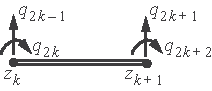
\includegraphics{Figure_17-23.pdf}
\caption{Generalized nodal displacements.\label{fig17.23}}
\end{wrapfigure}
See figure~\ref{fig17.23}. Admissible functions $v(z)$ and its derivative must be continuous within an element and be continuous between elements. Interpolation functions that satisfy these continuity requirements are Hermite cubic interpolation functions, which are denoted by $\phi_{i}(\zeta)$,. $i=1,2,3,4$. These interpolation functions are
\begin{align}\label{eq17.140}
\begin{array}{@{}ll@{}}\phi_{1}(\zeta)=\left(2-3 \zeta+\zeta^{3}\right)/4 & \phi_{2}(\zeta)=\left(h_{k}/ 8\right)\left(-1+\zeta+\zeta^{2}-\zeta^{3}\right) \\[4pt]\phi_{3}(\zeta)=\left(2+3 \zeta-\zeta^{3}\right)/4 & \phi_{4}(\zeta)=\left(h_{k}/8\right)\left(1+\zeta-\zeta^{2}-\zeta^{3}\right)\end{array}.
\end{align}
Let the derivative $\frac{d \phi_{i}}{d \zeta}$ be denoted by $\phi_{i}{ }^{\prime}$. The interpolation properties of the Hermite cubic functions are
\begin{align}\label{eq17.141}
\begin{array}{@{}cccc@{}}\phi_{1}(-1)=1 & \phi_{1}^{\prime}(-1)=0 & \phi_{1}(1)=0 & \phi_{1}^{\prime}(1)=0 \\[4pt]\phi_{2}(-1)=0 & \phi_{2}^{\prime}(-1)=-h_{k}/2 & \phi_{2}(1)=0 & \phi_{2}^{\prime}(1)=0 \\[4pt]\phi_{3}(-1)=0 & \phi_{3}^{\prime}(-1)=0 & \phi_{3}(1)=1 & \phi_{3}^{\prime}(1)=0 \\[4pt]\phi_{4}(-1)=0 & \phi_{4}^{\prime}(-1)=0 & \phi_{4}(1)=0 & \phi_{4}^{\prime}(1)=-h_{k}/2\end{array}.
\end{align}

{\def\thefigure{17.24}
\processfigure{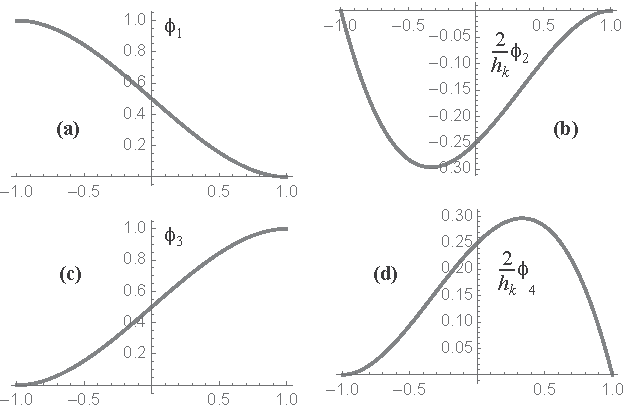
\includegraphics{Figure_17-24.pdf}
}{\caption{Hermite cubic interpolation functions.
(a)\break $\Phi_\textbf{1} (\zeta)$,
(b) $\frac{\textbf{2}}{h_k} \Phi_\textbf{2}(\zeta)$,
(c)\break $\Phi_\textbf{3} (\zeta)$, and
(d) $\frac{\textbf{2}}{h_k} \Phi_\textbf{4}(\zeta)$.\break
where $-\textbf{1}\leq \zeta \leq \textbf{1}$.\label{fig17.24}}}}


\noindent Graphs of Hermite cubic functions are shown in figure~\ref{fig17.24}. The displacement for element $\Omega_{\textrm{k}}$ is $v^{(k)}(\zeta)=[N(\zeta)]\left\{q^{(k)}\right\}$, where $[N(\zeta)]$ is the 1X4 matrix of interpolation functions, and $\left\{q^{(k)}\right\}$ is the 4X1 vector of the generalized displacements at the nodes. The interpolation matrix and nodal displacement vector are
\begin{align}\label{eq17.142}
[N(\zeta)]=\left[\phi_{1}(\zeta) \phi_{2}(\zeta) \phi_{3}(\zeta) \phi_{4}(\zeta)\right], \textrm{ and } \left\{q^{(k)}\right\}=\left[\begin{array}{@{}llll@{}} q_{2 k-1} & q_{2 k} & q_{2 k+1} & q_{2 k+2}\end{array}\right]^{T}.
\end{align}
The virtual displacement is $\bar{v}(\zeta)=[N(\zeta)]\{b\}$, where $\{b\}=\left[\begin{array}{@{}llll@{}}b_{1} & b_{2} & b_{3} & b_{4}\end{array}\right]^{T}$. The second derivative of the displacement, or curvature $\kappa$ of the centroidal axis in bending, is expressed as
\begin{gather}
\kappa=-\left(\frac{d^{2} v}{d z^{2}}\right)=-\left(\frac{d^{2} v}{d \zeta^{2}}\right)\left(\frac{2}{h_{k}}\right)^{2}=-\left(\frac{2}{h_{k}}\right)^{2} \frac{d^{2}}{d \zeta^{2}}[N(\zeta)]\left\{q^{(k)}\right\}=\left[N_{\kappa}(\zeta)\right]\big\{q^{(k)}\big\}, \textrm{ where}\label{eq17.143}\\
\left[N_{\kappa}(\zeta)\right]=\frac{1}{h_{k}^{2}}\left[\begin{array}{@{}llll@{}} -6 \zeta & h_{k}(-1+3 \zeta) & 6 \zeta & h_{k}(1+3 \zeta)\end{array}\right].
%\left[-6 \zeta h_{k}(-1+3 \zeta) 6 \zeta h_{k}(1+3 \zeta)\right]. \label{eq17.144}
\end{gather}
The the virtual curvature is $\bar{\kappa}=-\left(\frac{d^{2} \bar{v}^{(k)}}{d z^{2}}\right)=\left[N_{\kappa}(\zeta)\right]\{b\}=\{b\}^{T}\left[N_{\kappa}(\zeta)\right]^{T}$. The bilinear form evaluates as
\begin{align}\label{eq17.145}
B[v, \bar{v}]=\int_{0}^{L}\left(\bar{\kappa} E I_{x x} \kappa\right) d z=\{b\}^{T}\left(\int_{-1}^{1}\left[N_{\kappa}(\zeta)\right]^{T} E I_{x x}\left[N_{\kappa}(\zeta)\right] \frac{h_{k}}{2} d \zeta\right)\big\{q^{(k)}\big\}=\{b\}^{T}[K]\big\{q^{(k)}\big\}.
\end{align}
The element stiffness matrix is
\begin{align}\label{eq17.146}
[K]=\frac{E I_{x x}}{h_{k}^{3}}\left[\begin{array}{@{}cccc@{}}12 & -6 h_{k} & -12 & -6 h_{k} \\-6 h_{k} & 4 h_{k}^{2} & 6 h_{k} & 2 h_{k}^{2} \\-12 & 6 h_{k} & 12 & 6 h_{k} \\-6 h_{k} & 2 h_{k}^{2} & 6 h_{k} & 4 h_{k}^{2}\end{array}\right].
\end{align}

\vspace*{-1pc}

Referring to Fig.~\ref{fig17.16} on page~\pageref{fig17.16}, we express the boundary terms in the external virtual work (\ref{eq17.138}) as
\begin{align}
\left.\bar{v} V_{y}\right|_{z_{k+1}}-\left.\bar{v} V_{y}\right|_{z_{k}}+\left.\left(-\frac{d \bar{v}}{d z}\right) M_{x}\right|_{z_{k+1}}-\left.\left(-\frac{d \bar{v}}{d z}\right) M_{x}\right|_{z_{k}}&=b_{3} Q_{2 k+1}-b_{1}\left(-Q_{2 k-1}\right)+b_{4} Q_{2 k+2}-b_{2}\left(-Q_{2 k}\right) \nonumber \\
&=\{b\}^{T}\big\{Q^{(k)}\big\}. \label{eq17.147}
\end{align}
The prescribed distributed load terms in the external virtual work are
\begin{align}\label{eq17.148}
\int_{0}^{L}\hspace*{-2.5pt} f_{y} \bar{v} d z+\int_{0}^{L}\left[E I_{x x}\left(-\frac{d^{2} \bar{v}}{d z^{2}}\right)\right] \alpha \tau_{y} d z=\{b\}^{T}\left(\int_{-1}^{1} f_{y}^{(k)}[N(\zeta)]^{T} \frac{h_{k}}{2} d \zeta+\int_{-1}^{1} E I_{x x}\left[N_{k}(\zeta)\right]^{T} \alpha \tau_{y}^{(k)}(\zeta) \frac{h_{k}}{2} d \zeta\right),
\end{align}
where the distributed loading in the element is
\begin{align}\label{eq17.149}
f_{y}^{(k)}=f_{y}\left[\eta_{1}(\zeta) z_{k}+\eta_{2}(\zeta) z_{k+1}\right] \quad \tau_{y}^{(k)}=\tau_{y}\left[\eta_{1}(\zeta) z_{k}+\eta_{2}(\zeta) z_{k+1}\right].
\end{align}
The final result for the external virtual work for element $\Omega_{\textrm{k}}$ is
\begin{gather}
F[\bar{v}]=\{b\}^{T}\left(\left\{Q^{k}\right\}+\big\{F^{(k)}\big\}\right), \textrm{ where}\label{eq17.150}\\
\big\{Q^{(k)}\big\}=\left[\begin{array}{@{}llll@{}}Q_{2 k-1} & Q_{2 k} & Q_{2 k+1} & Q_{2 k+2}\end{array}\right]^{T} \textrm{ and } \left\{F^{(k)}\right\}=\left[\begin{array}{@{}llll@{}}F_{2 k-1} &F_{2 k} &F_{2 k+1} &F_{2 k+2}\end{array}\right]^{T}. \label{eq17.151}
\end{gather}
Explicit expressions for the components of the generalized force vector from the distributed load are
\begin{gather}
F_{2 k-1}=\int_{-1}^{1}\left[f_{y}^{(k)}(\zeta)\right] \phi_{1}(\zeta) \frac{h_{k}}{2} d \zeta+\int_{-1}^{1}\left[E I_{x x}\left(\frac{-6 \zeta}{h_{k}^{2}}\right)\right]\left[\alpha \tau_{y}^{(k)}(\zeta)\right] \frac{h_{k}}{2} d \zeta, \label{eq17.152} \\
F_{2 k}=\int_{-1}^{1}\left[f_{y}^{(k)}(\zeta)\right] \phi_{2}(\zeta) \frac{h_{k}}{2} d \zeta+\int_{-1}^{1}\left[E I_{x x} \frac{(-1+3 \zeta)}{h_{k}}\right]\left[\alpha \tau_{y}^{(k)}(\zeta)\right] \frac{h_{k}}{2} d \zeta, \label{eq17.153} \\
F_{2 k+1}=\int_{-1}^{1}\left[f_{y}^{(k)}(\zeta)\right] \phi_{3}(\zeta) \frac{h_{k}}{2} d \zeta+\int_{-1}^{1}\left[E I_{x x}\left(\frac{6 \zeta}{h_{k}^{2}}\right)\right]\left[\alpha \tau_{y}^{(k)}(\zeta)\right] \frac{h_{k}}{2} d \zeta, \textrm{ and}\label{eq17.154} \\
F_{2 k+2}=\int_{-1}^{1}\left[f_{y}^{(k)}(\zeta)\right] \phi_{4}(\zeta) \frac{h_{k}}{2} d \zeta+\int_{-1}^{1}\left[E I_{x x} \frac{(1+3 \zeta)}{h_{k}}\right]\left[\alpha \tau_{y}^{(k)}(\zeta)\right] \frac{h_{k}}{2} d \zeta. \label{eq17.155}
\end{gather}

\begin{thebibliography}{}\label{sec17.5}
\bibitem{} Bathe, K-J. \textit{\textbf{Finite Element Procedures in Engineering Analysis}}. Englewood Cliffs, NJ: Prentice-Hall, Inc., 1982, p. 167.

\bibitem{} Guyan, R.J. ``Reduction of Stiffness and Mass Matrices.'' \textit{\textbf{AIAA Journal}} 3, no.2, (1965): 380.

\bibitem{} Huebner, K. H., E. A.Thornton, and T. G. Byrom. \textit{\textbf{The Finite Element Method for Engineers}}. 3d ed.New York: John Wiley \& Sons, Inc., 1995.\label{Huebner}

\bibitem{} Irons, B,M. ``Structural Eigenvalue Problems: Elimination of Unwanted Variables.'' \textit{\textbf{AIAA Journal}} 3, no.5 (1965): 961--962

\bibitem{} Reddy, J. N. \textit{\textbf{An Introduction to the Finite Element Method}}, 4th ed. New York: McGraw Hill-Education, 2019.\label{Reddy}

\bibitem{} Szabo, B., and I. Babuska. \textit{\textbf{Finite Element Analysis}}. New York: John Wiley \& Sons, Inc., 1991.\label{SzaboBabuska}
\end{thebibliography}

\end{document} 